\documentclass[conference]{IEEEtran}
\IEEEoverridecommandlockouts
\usepackage{cite}
\usepackage{amsmath,amssymb,amsfonts}
\usepackage{graphicx}
\usepackage{textcomp}
\usepackage{xcolor}
\usepackage{booktabs}
\usepackage{url}
\renewcommand{\ttdefault}{cmtt}   % use Computer Modern typewriter (TFMs always present)
\def\BibTeX{{\rm B\kern-.05em{\sc i\kern-.025em b}\kern-.08em
    T\kern-.1667em\lower.7ex\hbox{E}\kern-.125emX}}

\begin{document}

\title{Operating Envelopes for Memristor Crossbar\\
Non-Idealities: A Calibrated Simulation Study from\\
Device Physics to In-Situ Learning}

\author{\IEEEauthorblockN{Jyotirmoy Ray}
\IEEEauthorblockA{\textit{Wipro Research} \\
Bengaluru, India \\
jyotirmoy.ray@wipro.com}
}

\maketitle

\begin{abstract}
Analog memristor crossbars promise large energy savings for neural-network
inference by performing matrix-vector multiplication in place, but their
practical accuracy is governed by device and circuit non-idealities. We build a
single, physically grounded compact model of an oxide valence-change cell,
calibrate it to a published self-rectifying Ag\textsubscript{2}O device, and
scale it, without changing any equation, from one device up to a 64x64 crossbar
and a small trained network. Using one consistent model
we reproduce the pinched current-voltage hysteresis and its collapse with sweep
frequency, quantify device-to-device variability across 4096 cells, solve the
full wire-resistance network with modified nodal analysis, and model thermally
activated retention loss. We then study three questions about how these effects
interact with computation; all headline numbers are averaged over multiple
seeds. First, closed-loop program-verify writing suppresses the accuracy loss
from variability (a 64 to 10 classifier recovers from 88.3 to 96.5 percent over
five seeds, matching a 96.5 percent software baseline). Second, finite wire
resistance scales sharply with array size (the mean output error of an
all-low-resistance array rises from 19 to 92 percent from 16x16 to 128x128 at
2.5 ohm per cell, and a realistic mixed-state map roughly halves these numbers).
Third, wire resistance is a static, structured distortion that on-chip training
can largely absorb: a two-spiral network deployed naively under IR drop sits at
63.5 percent and a cheap output calibration recovers only to 69.3 percent, but
training with the IR-drop network in the forward pass recovers it to 92.4
percent, whereas thermally activated retention drift, being time varying,
degrades a trained network to chance within weeks at 85 degrees Celsius and
cannot be trained away. Under this model the three non-idealities tend to
separate by remedy: variability is correctable at write time, IR drop is
absorbable by training (and not by output calibration alone), and retention is
only deferrable by rewriting. Calibrated to the published device, our simulator reproduces its measured 96.08
percent MNIST accuracy to within about one point (94.8 percent), and an
established hardware-aware toolkit (AIHWKit) agrees (95.4 percent). We then chart
operating envelopes over array size, wire resistance, and temperature that
delineate where each remedy is needed, and an energy model showing 18 to 41
TOPS/W (versus about 4 for a digital baseline) bounded by the same IR-drop limit.
The individual phenomena are established in prior work; our contribution is the
calibrated, baselined, seed-averaged study and the operating envelopes that make
the remedy boundaries explicit and quantitative. All experiments run in minutes
on a laptop CPU and the code is publicly available on GitHub.
\end{abstract}

\begin{IEEEkeywords}
memristor, RRAM, crossbar array, in-memory computing, analog computing, device
variability, IR drop, retention, in-situ training, neuromorphic.
\end{IEEEkeywords}

\section{Introduction}
The dominant energy cost of neural-network inference on conventional hardware is
not arithmetic but data movement: weights are shuttled between memory and a
separate arithmetic unit across a bus, the von Neumann bottleneck. Analog
resistive crossbars remove this cost by storing each weight as the conductance
of a nonvolatile device at the intersection of a wordline and a bitline. When
input voltages are applied to all wordlines at once, Ohm's law turns each device
into an analog multiplier and Kirchhoff's current law sums the products along
each bitline, so a full matrix-vector multiply (MVM) completes in a single read,
in place, with no per-element fetch \cite{ielmini2018, yu2018}.

Aluminium oxide (AlO\textsubscript{x}) and related transition-metal oxides
implement this conductance as a filamentary valence-change effect: an applied
field drives oxygen vacancies into or out of a conductive filament bridging two
electrodes, switching the cell between a low-resistance state (LRS) and a
high-resistance state (HRS) \cite{ielmini2016}. The same physics that makes the
device a nonvolatile memory also makes it an imperfect computing element. Three
non-idealities dominate in practice: device-to-device and cycle-to-cycle
variability, finite wordline and bitline wire resistance that causes an IR
voltage drop across the array, and thermally activated relaxation of the stored
state (retention loss). A large literature reports each effect and proposes
point mitigations, and several landmark demonstrations have trained networks
directly on hardware to tolerate them \cite{prezioso2015, yao2020, li2018}.

What is often missing, especially for a newcomer to the field, is a single,
internally consistent account that runs from the device current-voltage curve up
to a trained network and treats the three non-idealities on the same footing so
that their distinct characters become visible. This paper provides that account.
We deliberately use one device model everywhere and add each non-ideality as a
small, named extension, so that every system-level number can be traced back to a
device equation. Our contributions are:

\begin{enumerate}
\item A compact AlO\textsubscript{x} valence-change model (one state variable,
threshold-gated switching, ohmic LRS blended with a nonlinear HRS) that
reproduces the pinched hysteresis loop, its frequency-dependent collapse, and
analog multilevel states, and that vectorizes unchanged to a 4096-cell array
(Section \ref{sec:device}, \ref{sec:array}).
\item A full crossbar IR-drop solver based on modified nodal analysis (MNA) of
the $2NM$-node resistive network, used to quantify how MVM error grows with array
size (Section \ref{sec:irdrop}).
\item An Arrhenius retention model and a controlled, seed-averaged comparison
that places the three non-idealities on one footing and shows how they separate
by remedy under this model: variability is removed by closed-loop programming, IR
drop is absorbed by hardware-in-the-loop training, and retention is only
deferrable (Sections \ref{sec:retention}, \ref{sec:insitu}, \ref{sec:discussion}).
\item A reproducible demonstration, with a baseline, that on-chip training
recovers a network from 63.5 to 92.4 percent under wire resistance, while a cheap
output calibration recovers only to 69.3 percent (so the recovery is not a
calibration artifact), and a matched demonstration that the same training is
powerless against retention drift (Section \ref{sec:insitu}).
\item Calibration of the model to a published self-rectifying Ag\textsubscript{2}O
crossbar \cite{keshari2026} (reproducing its measured MNIST accuracy, cross-checked
against AIHWKit), two-dimensional \emph{operating envelopes} that map where each
remedy is needed in (array size, wire resistance) and (time, temperature), and an
energy model (Section \ref{sec:envelope}).
\end{enumerate}

We stress what is and is not new. Each phenomenon here is established:
program-verify mitigates programming variability; IR drop grows with array size,
conductance density and wire resistance; in-situ and hardware-aware training
absorb crossbar non-idealities including wire resistance \cite{prezioso2015,
liNComm2018, he2019, rasch2023}; and retention loss requires refresh or
drift-aware compensation \cite{joshi2020}. Our contribution is not a new
mechanism but a single consistent model used end-to-end, multi-seed evidence,
and an explicit calibration baseline, so that the differing characters of the
three effects become visible in one place. This is a simulation study with an
intentionally simplified model; the goal is reproducible clarity, not
silicon-accurate prediction. Limitations are in Section \ref{sec:limitations}.
All code and scripts to reproduce every figure and number in this paper are
available at \url{https://github.com/rayjyotir5/alox-crossbar-nonidealities}.

\section{Background and Related Work}
\label{sec:relwork}
\textbf{Memristors and RRAM.} The memristor was posited by Chua as the fourth
passive element linking charge and flux \cite{chua1971} and connected to
thin-film oxide devices by Strukov et al. \cite{strukov2008}. Practical resistive
RAM (RRAM) cells switch by forming and rupturing conductive filaments; Ielmini
and others review the mechanisms, reliability, and scaling
\cite{ielmini2016, ielmini2018}. Compact models such as the Yakopcic model
\cite{yakopcic2011} capture the nonlinear conduction and threshold switching that
we adopt in reduced form.

\textbf{Crossbar accelerators.} Architectures including ISAAC \cite{shafiee2016}
and PRIME \cite{chi2016} use RRAM crossbars as MVM engines for deep networks,
and fully hardware-implemented memristor convolutional networks have been
demonstrated \cite{yao2020}, along with large-scale analog signal and image
processing \cite{li2018}. Recent experimental passive crossbars are directly
comparable in scale to our simulation: Keshari et al. fabricate a self-rectifying
Ag-oxide 64x64 array with multilevel conductance ($\sim$3.6 to 22.3 $\mu$S) and
report 96.08 percent MNIST accuracy under device constraints, using
self-rectification to suppress the sneak-path and IR-drop problems we quantify
\cite{keshari2026}. These works also document the non-idealities that motivate
ours.

\textbf{In-situ and hardware-aware training.} Prezioso et al. trained a
single-layer perceptron directly on a metal-oxide memristor array
\cite{prezioso2015}, and Li et al. demonstrated efficient self-adaptive in-situ
learning in multilayer memristor networks \cite{liNComm2018}, both establishing
that training in the loop tolerates device imperfection. Hardware-aware training
that models non-idealities (including wire IR drop) during training and adapts
the network around them is now standard: He et al. inject modeled ReRAM
non-ideal effects during mapping \cite{he2019}, and Rasch et al. scale
hardware-aware training across large DNNs and a broad set of analog in-memory
non-idealities \cite{rasch2023}. Drift-aware inference for phase-change memory is
likewise established \cite{joshi2020}. Our hardware-in-the-loop IR-drop result is
firmly in this tradition; we do not claim the phenomenon, but we add a controlled
calibration baseline and seed statistics within a single device-to-system model,
and we contrast it explicitly with retention, which the same loop cannot fix.

\section{From a Memristor to a Learning Array}
\label{sec:device}
\subsection{How a memristor works}
A resistor obeys $I=V/R$ with $R$ fixed, so its current-voltage curve is a single
straight line with no memory. Chua's argument for a fourth fundamental element
\cite{chua1971} is that a device can instead link flux and charge, making its
resistance depend on the history of charge that has passed through it: the
memristor remembers. In an oxide cell this memory is physical. The film between
the two electrodes is normally insulating, but a sufficient field drives charged
oxygen vacancies into a conductive filament that bridges the electrodes; a reverse
field ruptures it. A complete filament is the low-resistance state (LRS), a
ruptured one the high-resistance state (HRS), and partial filaments give a
continuum of analog states in between.

Three consequences follow, and they are the spine of this paper. First, because
moving ions takes a threshold field and finite time, a slow voltage sweep traces
a \emph{pinched hysteresis loop}: the resistance on the way up differs from the
way down, yet both branches pass through the origin because no current flows at
zero voltage (Section \ref{sec:res-device}). Second, when the voltage returns to
zero the filament stays put, held by an energy barrier, so the conductance is a
\emph{nonvolatile stored value}; raising temperature lowers that barrier and the
state slowly relaxes, which is retention loss (Section \ref{sec:retention}).
Third, that stored conductance is exactly what a neural network needs as a
\emph{weight}, and an array of such cells multiplies an input vector by a weight
matrix in one electrical step (Section \ref{sec:array}). The rest of the paper
builds on these three facts in order: the device, then the array and its
non-idealities, then inference, then on-chip learning.

\subsection{Compact device model}
We model the cell with a single internal state variable $w \in [0,1]$ that
represents filament completeness: $w \to 1$ is the LRS (filament bridges the
oxide) and $w \to 0$ is the HRS (filament ruptured). The terminal current blends
an ohmic LRS branch with a sinh-nonlinear HRS branch, the behaviour AlO\textsubscript{x}
cells show on a parameter analyzer:
\begin{equation}
I(V,w) = w\,\frac{V}{R_\mathrm{on}} + (1-w)\,\frac{V_0}{R_\mathrm{off}}\sinh\!\left(\frac{V}{V_0}\right),
\label{eq:conduct}
\end{equation}
where $R_\mathrm{on}$ and $R_\mathrm{off}$ are the LRS and HRS resistances and
$V_0$ shapes the HRS nonlinearity. The state evolves only when the bias exceeds
a SET or RESET threshold, which is the origin of both hysteresis and
nonvolatility:
\begin{equation}
\frac{dw}{dt} =
\begin{cases}
k_\mathrm{s}(V-V_\mathrm{set})\,(1-w^{p}), & V > V_\mathrm{set}\\[2pt]
-k_\mathrm{r}(-V-V_\mathrm{reset})\,(1-(1-w)^{p}), & V < -V_\mathrm{reset}\\[2pt]
0, & \text{otherwise.}
\end{cases}
\label{eq:state}
\end{equation}
The window factors $(1-w^{p})$ and $(1-(1-w)^{p})$ ease the dynamics near the
rails and produce the gradual, saturating, asymmetric conductance change between
potentiation (SET) and depression (RESET) that is characteristic of real cells
and central to in-situ learning. A small-signal read at a sub-threshold voltage
$V_\mathrm{read}$ leaves $w$ unchanged, so reading is nondestructive. Default
parameters are listed in Appendix \ref{app:params}.

\section{Crossbar Array and Non-Ideality Models}
\label{sec:array}
\textbf{Variability.} An $N\times N$ array instantiates Eq.~\ref{eq:conduct} and
\ref{eq:state} per cell with parameters drawn from realistic distributions:
log-normal $R_\mathrm{on}$ and $R_\mathrm{off}$ (15 and 30 percent spread, the
HRS being the more variable), and Gaussian SET and RESET thresholds. A
multiplicative cycle-to-cycle term perturbs each programming pulse.

\textbf{Differential weights.} Signed weights are mapped to a pair of cells,
$W \propto (G^{+}-G^{-})$, so that one bitline pair encodes positive and negative
contributions; this also cancels common-mode disturbances.

\textbf{Closed-loop programming.} To write a target conductance map we use
program-verify: read every cell, then apply a SET pulse to those below target and
a RESET pulse to those above, repeated until convergence. Residual error reflects
finite pulse granularity and write noise rather than raw device spread.

\textbf{Wire IR drop.}
\label{sec:irmodel}
We solve the full resistive network rather than assuming ideal Ohm-Kirchhoff
behaviour. Each cross-point contributes a row-wire node and a column-wire node;
adjacent nodes along a wire are joined by a segment conductance $g_w = 1/r_w$, and
the device $G_{ij}$ links the two node planes. Driving rows from their left ends
and grounding columns at their feet yields a $2NM$-unknown linear system assembled
by modified nodal analysis. Because the conductance matrix depends only on
$G$ and $r_w$, we factor it once (sparse LU) and reuse the factorization across
many input vectors, which makes hardware-in-the-loop training tractable.

\textbf{Retention.} The stored state relaxes toward equilibrium with an Arrhenius
time constant,
\begin{equation}
w(t) = w_\mathrm{eq} + (w_0-w_\mathrm{eq})\,e^{-t/\tau(T)},\quad
\tau(T)=\tau_0\,e^{E_a/k_BT},
\label{eq:retention}
\end{equation}
so a programmed LRS cell loses conductance over time, faster when hot. We use
$E_a=1.0$ eV.

\section{Experimental Setup}
All experiments use NumPy, SciPy (sparse LU for the IR-drop solve), scikit-learn
(the digit dataset and the reference classifier), and PyTorch (a reference
convolution), on a laptop CPU; the full pipeline runs in minutes. Code is
organised as a device-and-array module, a non-idealities module (IR drop,
retention, inference), and an in-situ learning module; see
Appendix \ref{app:repro}.

\section{Results}
\subsection{Single-Device Behaviour}
\label{sec:res-device}
Figure \ref{fig:device} shows a quasi-static triangular sweep. Panel (a) is the
pinched hysteresis loop, the defining memristor signature: both branches cross
the origin because $I=0$ whenever $V=0$. Panel (b) shows the state variable
switching abruptly at the SET and RESET thresholds, and holding flat elsewhere,
which is why a single voltage maps to two resistances (hysteresis) and why the
state survives at zero bias (memory). Panel (c) shows the loop collapsing as
sweep frequency rises: at 1, 10, and 100 Hz the peak state reaches 1.0, 0.65, and
0.09 respectively, because the ions cannot keep up and the device stops switching.

\begin{figure*}[t]
\centering
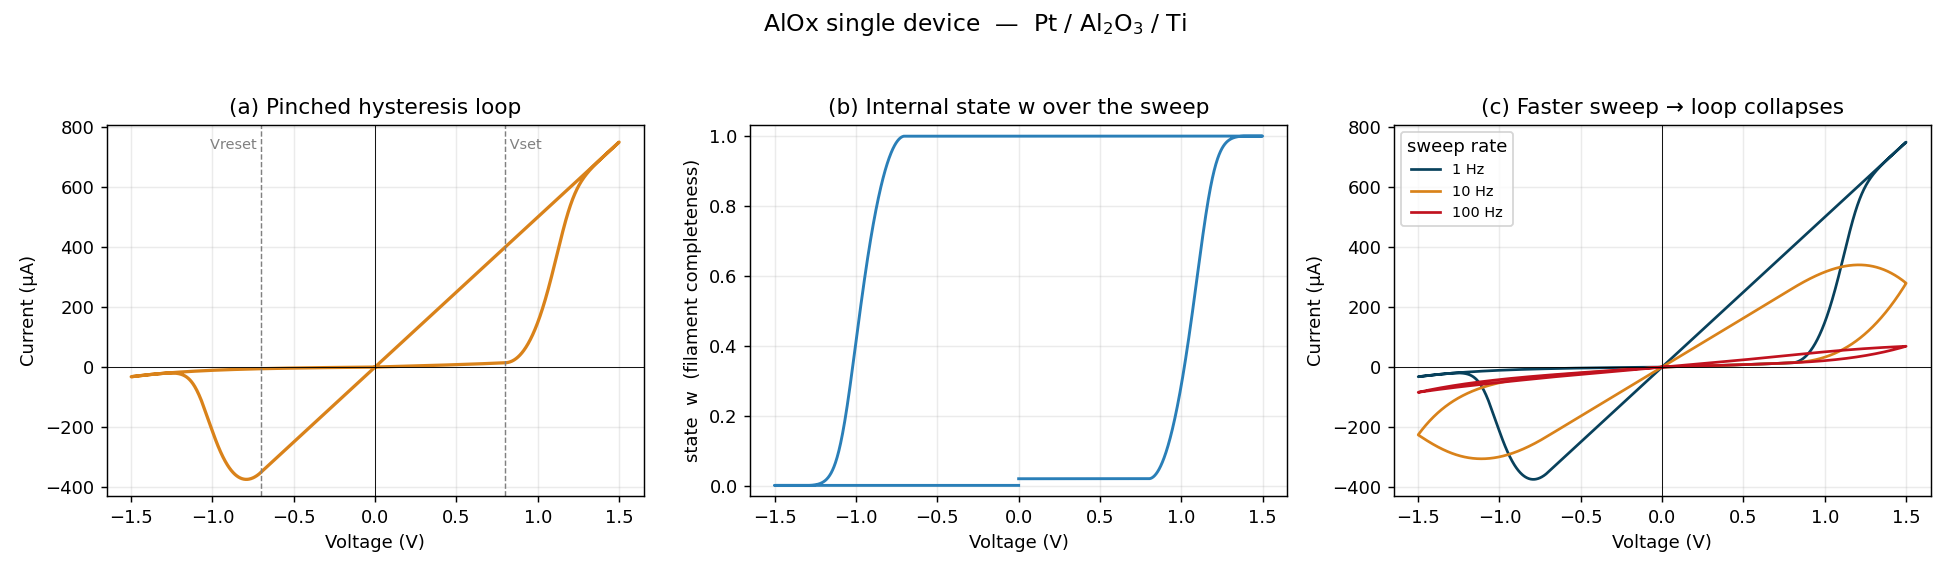
\includegraphics[width=0.98\textwidth]{figures/fig1_single_device.png}
\caption{Single AlO\textsubscript{x} cell. (a) Pinched hysteresis loop. (b) State
variable $w$ over the sweep, showing threshold-gated SET and RESET. (c) The loop
area collapses monotonically as sweep frequency increases and the state can no
longer fully switch.}
\label{fig:device}
\end{figure*}

\subsection{Array Variability}
\label{sec:res-var}
Driving all 4096 cells fully off and then fully on yields the conductance
histograms of Fig.~\ref{fig:var}(a). The HRS reads $7.09\,\mu$S
($\sigma/\mu=0.24$) and the LRS $199\,\mu$S ($\sigma/\mu=0.19$); although the
means differ by about 28x, the worst-case on/off read margin (lowest LRS over
highest HRS) is only about 4x. This margin erosion, not the mean ratio, is the
practical variability problem. Panel (b) overlays the loops of 60 random cells:
no two are identical.

\begin{figure*}[t]
\centering
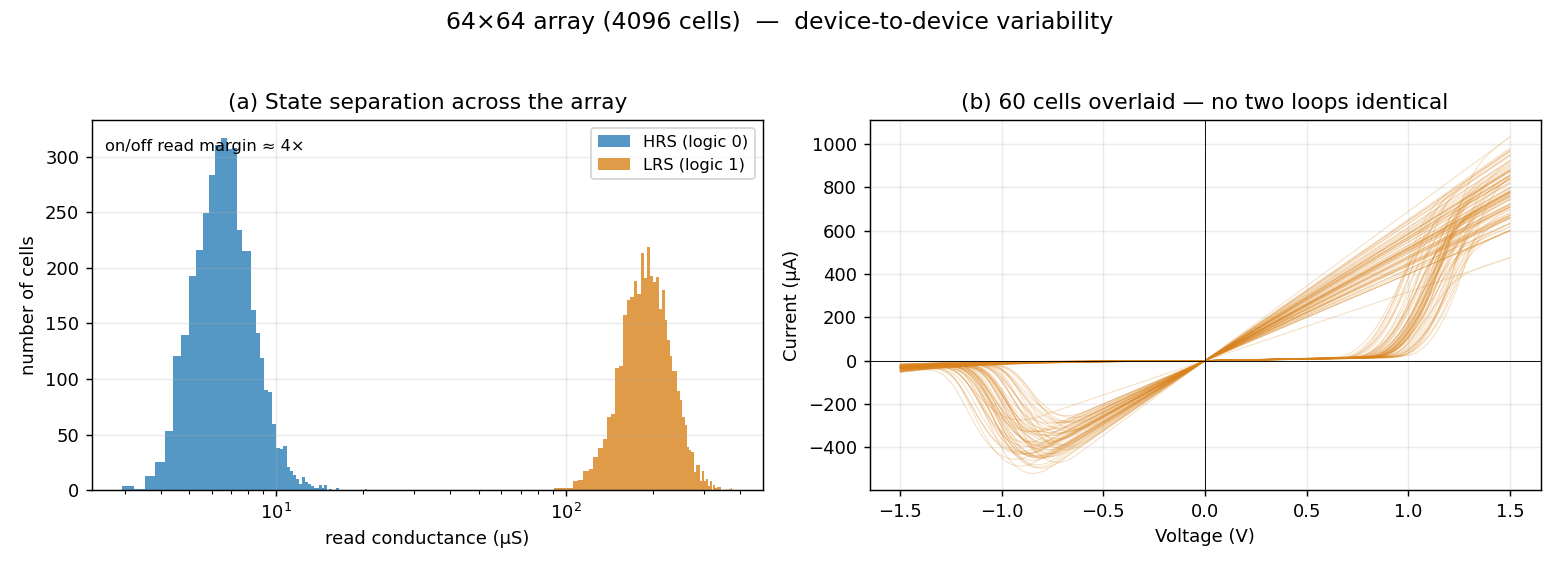
\includegraphics[width=0.98\textwidth]{figures/fig2_array_variability.png}
\caption{64x64 array (4096 cells). (a) HRS and LRS read-conductance
distributions; the worst-case on/off margin (about 4x) is far smaller than the
ratio of means (about 28x). (b) Current-voltage loops of 60 randomly chosen
cells, showing device-to-device spread.}
\label{fig:var}
\end{figure*}

\subsection{In-Memory MVM and Classifier Inference}
\label{sec:res-inf}
Figure \ref{fig:compute} programs an image into the array as a conductance map
and reads it back; the program-verify write achieves about 0.5 percent RMSE of
full scale. The analog MVM (input voltages times the programmed conductances,
summed by column) tracks an ideal digital MVM to about 0.5 percent mean error.

We then deploy a real classifier whose single layer fits the array. A logistic
regression on 8x8 handwritten digits (64 inputs, 10 classes) is trained in
software (96.5 percent test accuracy), mapped to differential conductances, and
evaluated on the array. Table \ref{tab:inference} reports the accuracy under each
condition. An ideal write reproduces the software accuracy, confirming the
pipeline. Open-loop writing (which lets device variation pass through
uncorrected) costs about 8 points ($88.3 \pm 2.6$ over five seeds), and
program-verify recovers essentially all of it ($96.5 \pm 0.3$). Adding wire IR
drop is then the larger loss. As a building-block check, a
single convolutional layer (the dominant operator in detectors such as YOLO)
mapped to the array reproduces a floating-point convolution with cosine
similarity 0.999, but a full detector neither fits in nor can be loaded onto a
single small tile, so we report the layer fidelity and the end-to-end classifier
rather than a detector.

\begin{table}[t]
\caption{Digit classifier (64 to 10) under array non-idealities
(5 seeds, mean $\pm$ std).}
\label{tab:inference}
\centering
\begin{tabular}{lc}
\toprule
Condition & Test accuracy (\%) \\
\midrule
Software (float) & 96.5 \\
Crossbar, ideal write & 96.5 \\
Open-loop write (raw variability) & $88.3 \pm 2.6$ \\
Program-verify write & $96.5 \pm 0.3$ \\
\quad + wire IR drop ($r_w=2.5\,\Omega$) & $75.1 \pm 1.0$ \\
\bottomrule
\end{tabular}
\end{table}

\begin{figure*}[t]
\centering
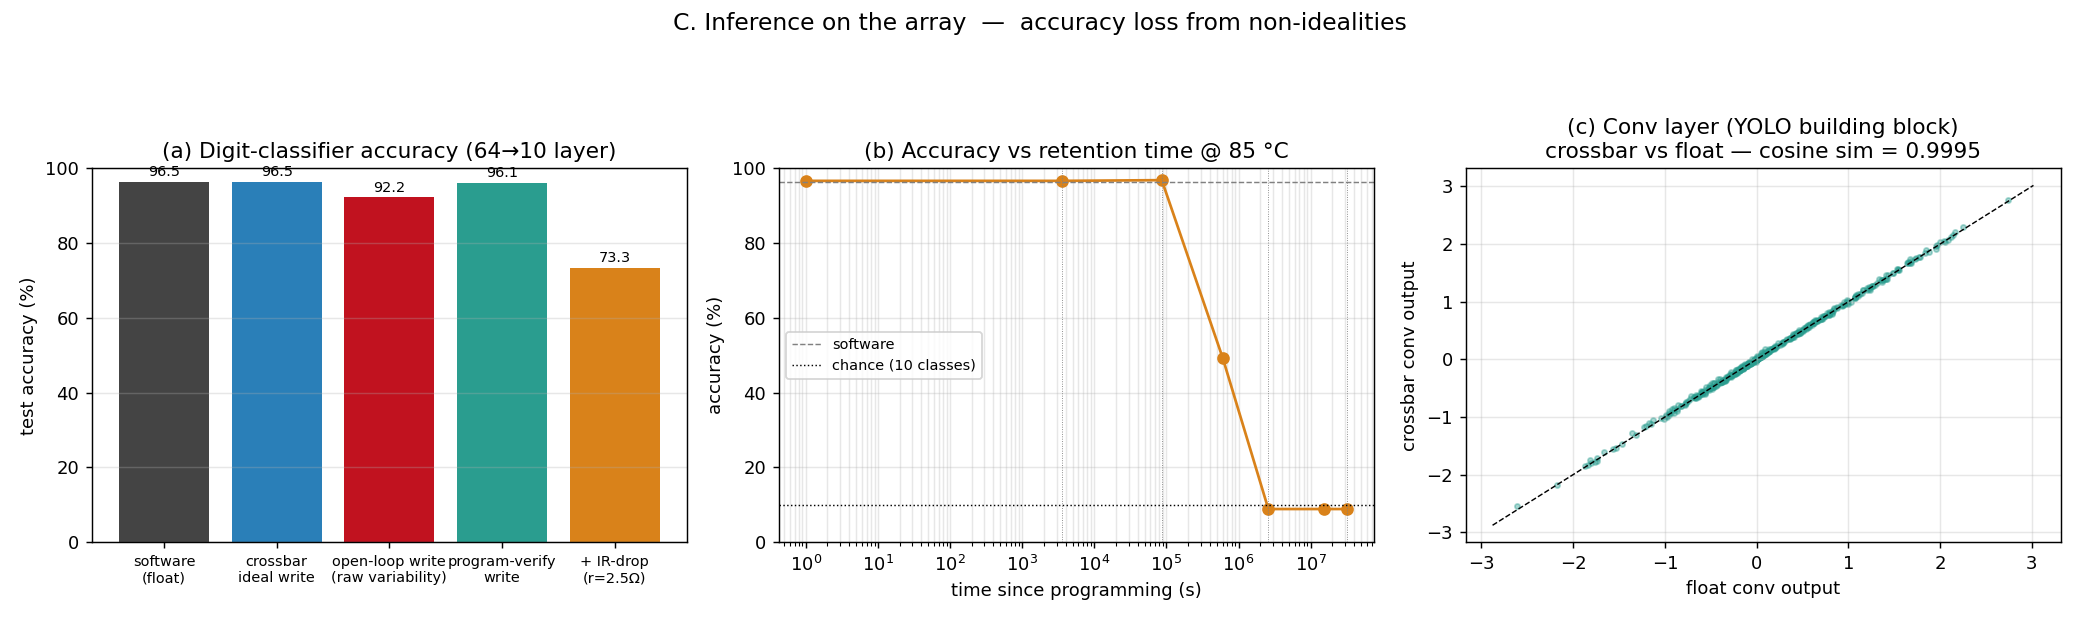
\includegraphics[width=0.98\textwidth]{figures/figC_inference.png}
\caption{Inference on the array. (a) Classifier accuracy across conditions:
variability costs accuracy, program-verify recovers it, and IR drop then
dominates. (b) Accuracy versus retention time at 85 degrees Celsius. (c) A
convolutional layer (a YOLO building block) on the array reproduces the
floating-point output with cosine similarity 0.999.}
\label{fig:inference}
\end{figure*}

\begin{figure*}[t]
\centering
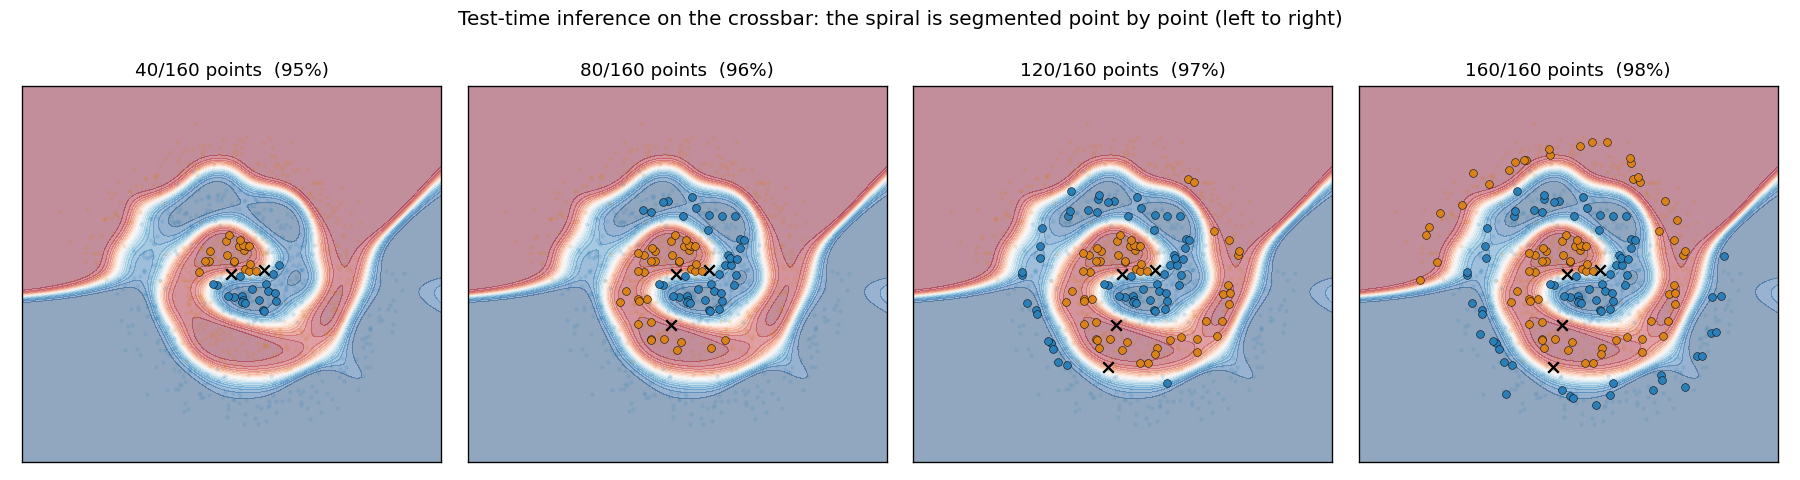
\includegraphics[width=0.98\textwidth]{figures/insitu_inference_strip.png}
\caption{Test-time inference unfolding in time (frames left to right). A held-out
spiral is pushed through the trained crossbar point by point (revealed from the
centre outward); each point is classified and placed on the plane, coloured by
the array's prediction (black cross if wrong), over the learned decision
boundary. By the last frame the two arms are cleanly separated.}
\label{fig:infstrip}
\end{figure*}

\subsection{Wire IR-Drop Scaling}
\label{sec:irdrop}
Figure \ref{fig:irdrop}(a) maps the wordline voltage across a 64x64 all-LRS array
driven at 200 mV: the voltage sags from the driven edge to about 50 mV at the far
corner, so distant cells are under-driven and contribute too little current.
Panel (b) and Table \ref{tab:irdrop} show that the resulting MVM error grows
sharply with array size, because both the wire length and the aggregate current
increase. This is the worst case (every cell in LRS); a realistic mixed-state
map roughly halves the error (for example 51.1 versus 75.5 percent at 64x64,
Table \ref{tab:irdrop}), but the monotone growth with size holds for both and
explains why passive arrays are size limited and why access transistors,
current limiting, or self-rectifying cells \cite{keshari2026} are used in
practice.

\begin{table}[t]
\caption{Mean MVM error (\%) vs.\ array size (5 seeds; std $<0.3$). All-LRS is
the worst case; mixed-state is a realistic random conductance map.}
\label{tab:irdrop}
\centering
\begin{tabular}{lcccc}
\toprule
Pattern, $r_w$ & 16x16 & 32x32 & 64x64 & 128x128 \\
\midrule
all-LRS, $1.0\,\Omega$ & 8.6 & 26.1 & 56.6 & 82.4 \\
all-LRS, $2.5\,\Omega$ & 18.8 & 46.1 & 75.5 & 91.5 \\
all-LRS, $5.0\,\Omega$ & 31.5 & 62.5 & 85.3 & 95.2 \\
mixed-state, $2.5\,\Omega$ & 6.9 & 22.1 & 51.1 & 79.0 \\
\bottomrule
\end{tabular}
\end{table}

\begin{figure*}[t]
\centering
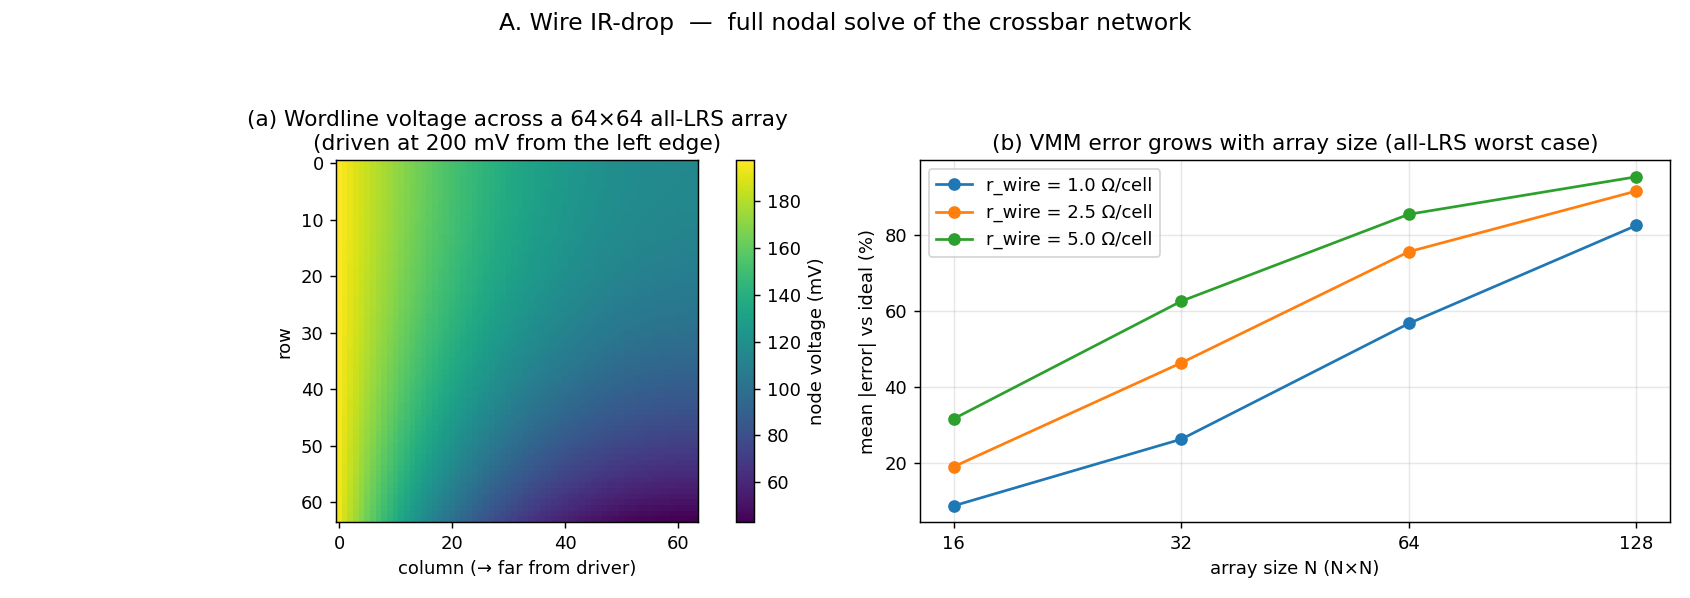
\includegraphics[width=0.98\textwidth]{figures/figA_irdrop.png}
\caption{Wire IR drop from the full nodal solve. (a) Wordline voltage across a
64x64 all-LRS array driven at 200 mV; the voltage droops toward the far corner.
(b) Mean MVM error versus array size for three wire resistances (worst case).}
\label{fig:irdrop}
\end{figure*}

\subsection{Retention}
\label{sec:retention}
Figure \ref{fig:retention}(a) shows normalized LRS conductance versus time at
four temperatures. The Arrhenius time constant is about 12 years at 25 degrees
Celsius, 6.5 days at 85 degrees, and 6 hours at 125 degrees. Panel (b)
illustrates a stored weight pattern fading to nothing over a month at 85 degrees:
the device forgetting in real time. The absolute time scale depends on the
activation energy: holding 25-degree retention near ten years, the 85-degree
time constant is 19.8, 5.4, and 1.5 days for $E_a = 0.8$, $1.0$, and $1.2$ eV
respectively, so the qualitative cliff is general while its location is set by
$E_a$ and temperature.

\begin{figure*}[t]
\centering
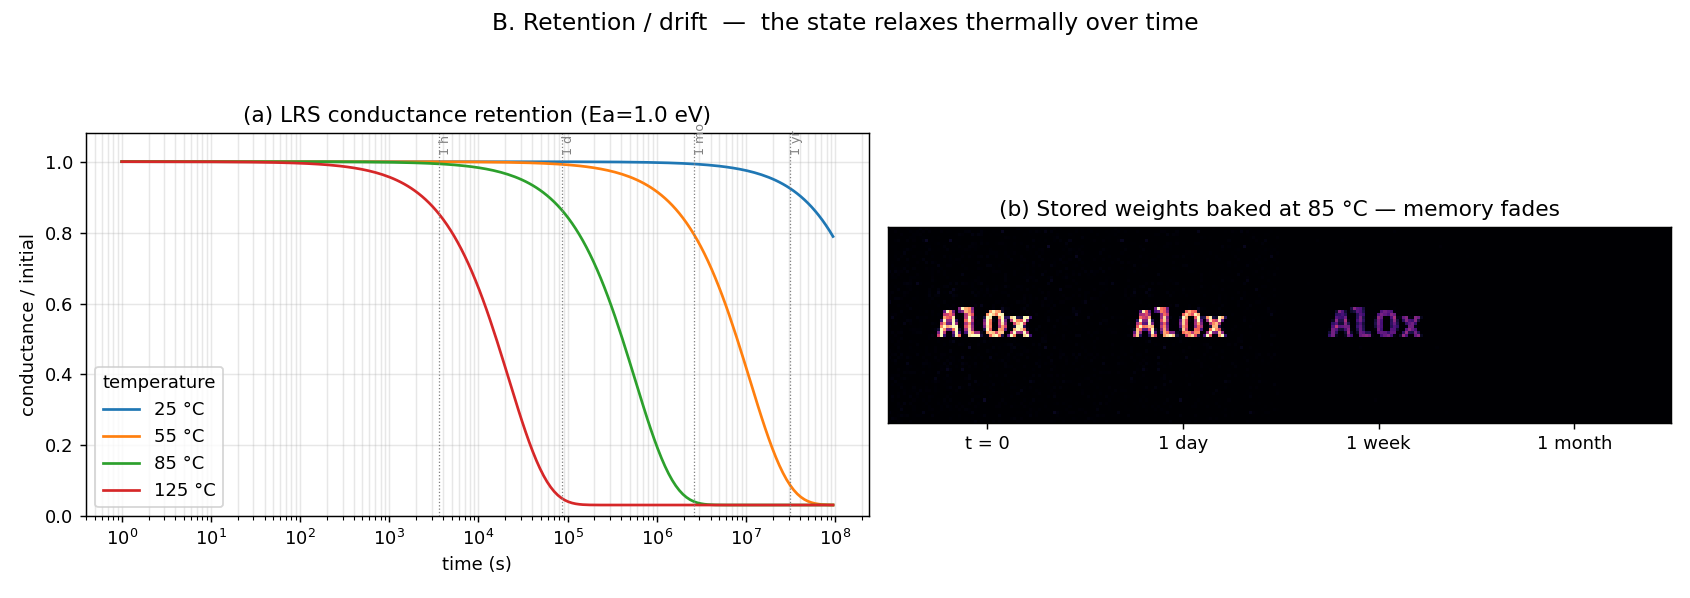
\includegraphics[width=0.98\textwidth]{figures/figB_retention.png}
\caption{Retention. (a) Normalized LRS conductance versus time at four
temperatures; each temperature shifts the decay by roughly a decade. (b) A
stored weight pattern baked at 85 degrees Celsius fades from sharp to gone over a
month.}
\label{fig:retention}
\end{figure*}

\subsection{In-Situ Learning and the Character of Each Non-Ideality}
\label{sec:insitu}
We now ask how the non-idealities interact with training, using a two-spiral
classification task that requires a genuinely nonlinear network (a linear model
scores about 50 percent). A 2-64-2 multilayer perceptron is trained with its
weights stored on differential crossbar tiles; every weight update is a
programming pulse that moves $w$ through the same nonlinear dynamics of
Eq.~\ref{eq:state}, so the update inherits the device's saturating, asymmetric,
variable response. We use a gradient-proportional pulse rule (pulse width scales
with the gradient magnitude).

\textbf{Training converges on imperfect devices.} The variable, noisy crossbar
network learns the task, but reliability depends on the pulse schedule. With a
fixed pulse size the spiral accuracy is seed-sensitive ($72.4 \pm 13.1$ over four
seeds); adding a pulse-size decay schedule stabilises it to $95.2 \pm 1.2$,
against a floating-point baseline near 95 percent. On an easier second nonlinear
task (concentric circles) training is robust either way ($99.9 \pm 0.1$).
Figure \ref{fig:insitu} shows a representative seed. Two mechanisms matter.
First, the usable weight range: the conductance window must encode weights up to
about $\pm 8$ for the spiral task, and clipping it to $\pm 3$ caps accuracy near
80 percent. Second, device noise helps: noiseless, identical devices stall in
limit cycles under deterministic nonlinear updates, whereas cycle-to-cycle noise
acts as beneficial dither, a known and somewhat counterintuitive in-situ result.

\begin{figure*}[t]
\centering
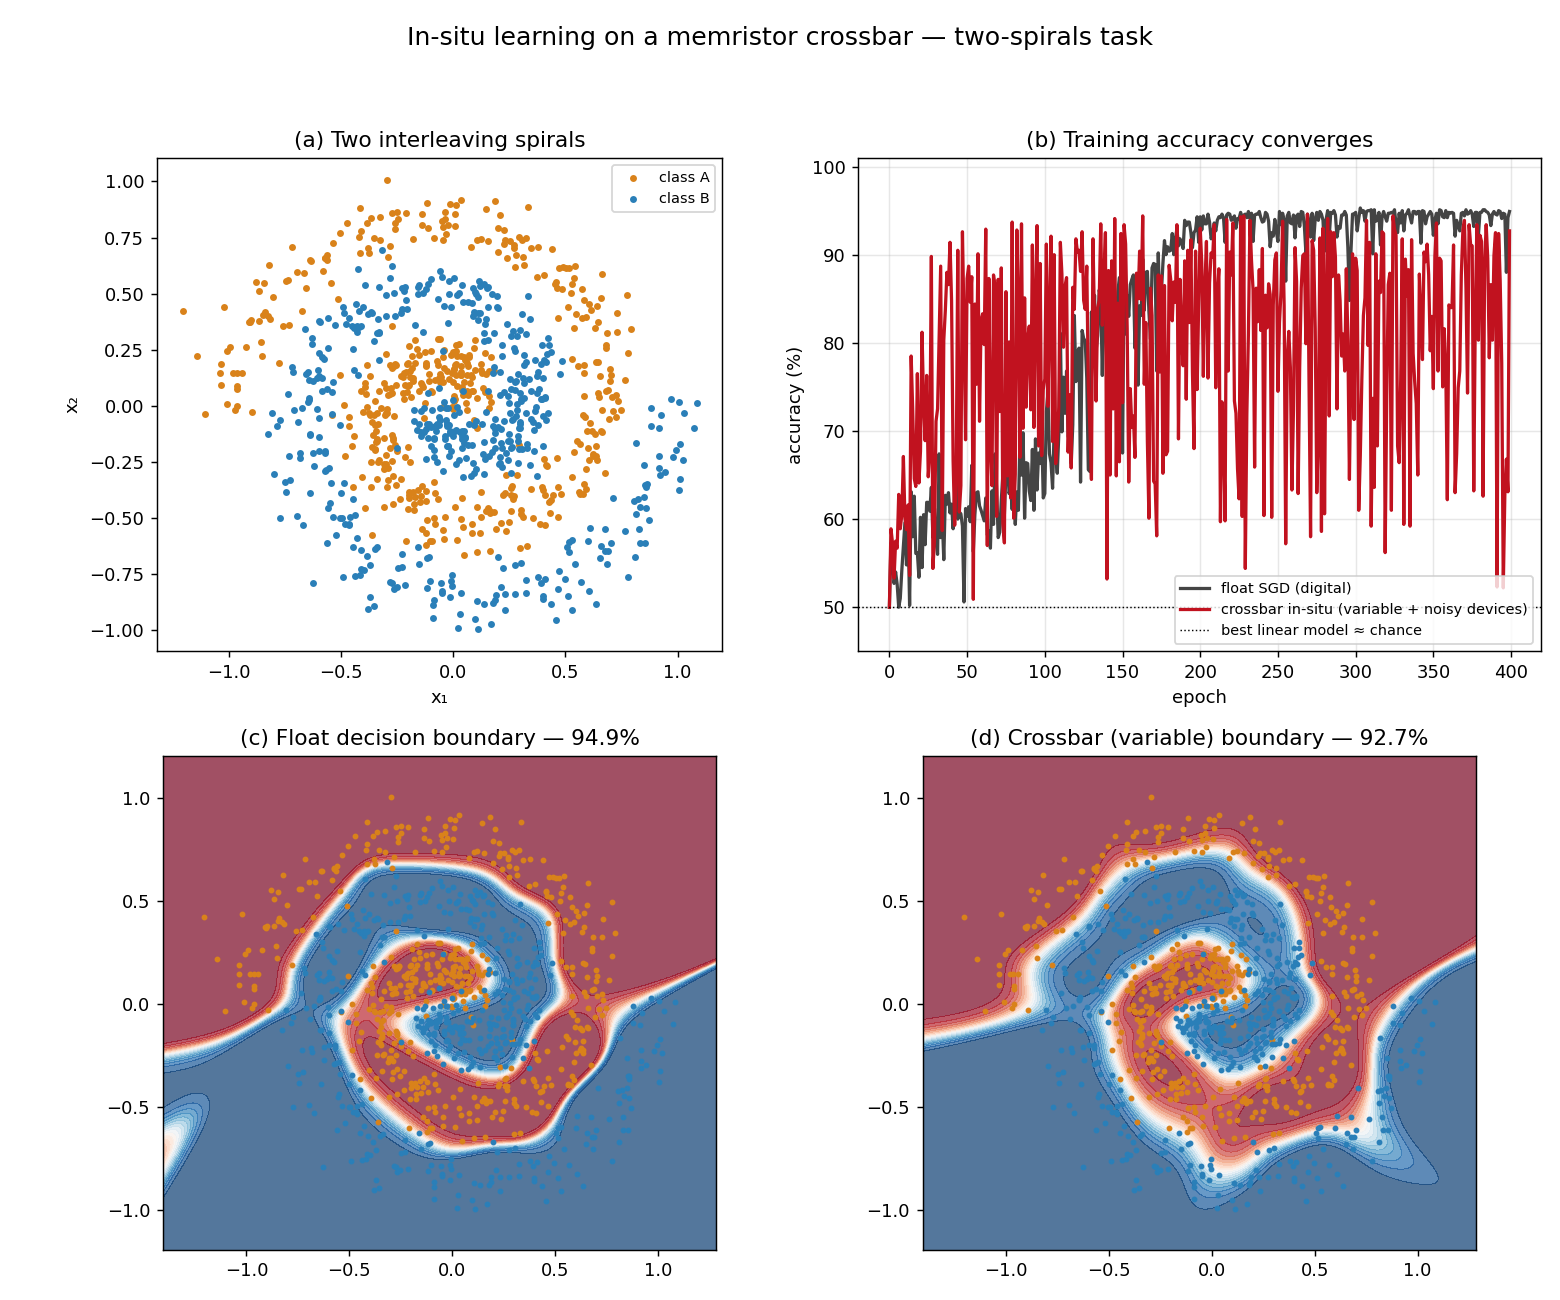
\includegraphics[width=0.92\textwidth]{figures/figD_insitu_learning.png}
\caption{In-situ learning on the crossbar (a representative seed; see text for
seed statistics). (a) The two-spiral task. (b) Training accuracy converges for
both floating-point SGD and the variable, noisy crossbar. (c, d) Learned decision
boundaries; the crossbar closely matches floating point.}
\label{fig:insitu}
\end{figure*}

\textbf{IR drop is absorbable by training, and not by calibration alone.} A
network trained with an ideal forward pass and then deployed through the IR-drop
network sits at $63.5 \pm 0.9$ percent at $r_w=1\,\Omega$ (three seeds). Training
the same network with the IR-drop network in the forward pass (gradients from an
ideal-weight surrogate, since one cannot backpropagate through the analog array)
recovers it to $92.4 \pm 0.9$ percent (Fig.~\ref{fig:drift}(b),(c)). To check that
this is genuine compensation and not a trivial output rescaling, we add a
baseline: fit a per-output affine map (gain and bias) from the IR-distorted
logits to the ideal logits on half the data and evaluate on the rest. This output
calibration recovers only to $69.3 \pm 1.5$ percent, far below the trained
$92.4$. So the recovery requires learning weights tuned to the distorted
transfer function, not a cheap post-hoc correction. A pulse-size decay schedule
is needed to settle the otherwise noisy convergence caused by the
surrogate-gradient mismatch.

\textbf{Retention is not.} Taking the trained network and letting its
conductances relax (Fig.~\ref{fig:drift}(a)), the accuracy holds for about a day
at 85 degrees, falls through 60 percent at one week, and reaches chance (50
percent) by one month. A static set of weights cannot resist this, because the
distortion is time varying rather than fixed; it is deferred by periodic
rewriting, or mitigated by drift-aware mapping, recalibration, or refresh
policies, but not removed by the one-time hardware-aware training that absorbs IR
drop.

\begin{figure*}[t]
\centering
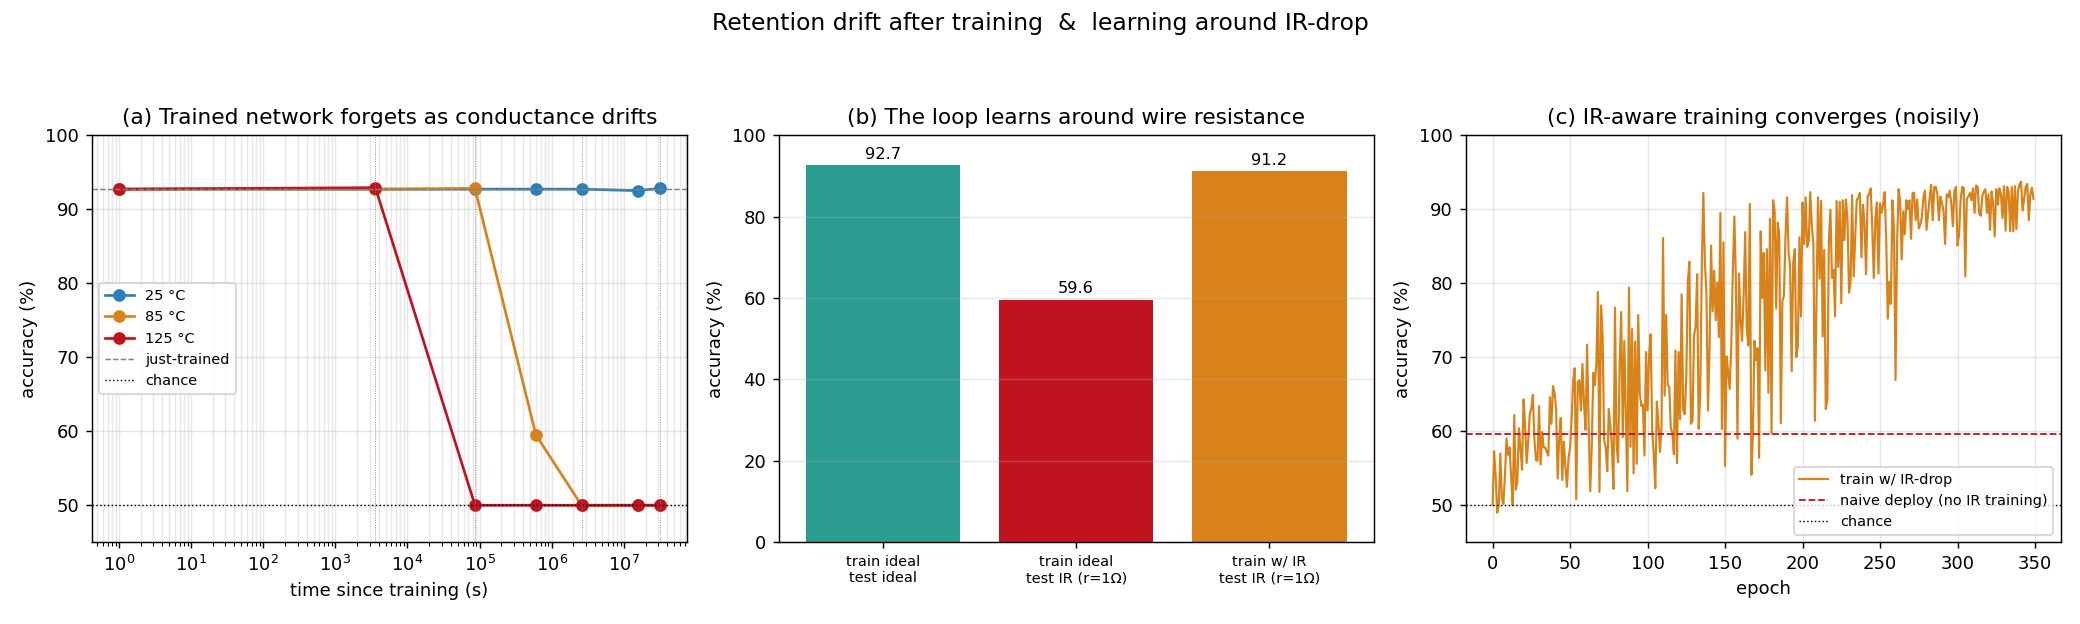
\includegraphics[width=0.98\textwidth]{figures/figE_drift_and_irdrop.png}
\caption{Two interactions of non-idealities with a trained network. (a) Retention
drift after training: accuracy holds for about a day at 85 degrees Celsius, then
dissolves to chance by one month. (b) IR drop: naive deployment under wire
resistance collapses accuracy, but training with IR drop in the loop recovers it.
(c) The IR-aware training converges (with a pulse-size decay schedule).}
\label{fig:drift}
\end{figure*}

\begin{figure*}[t]
\centering
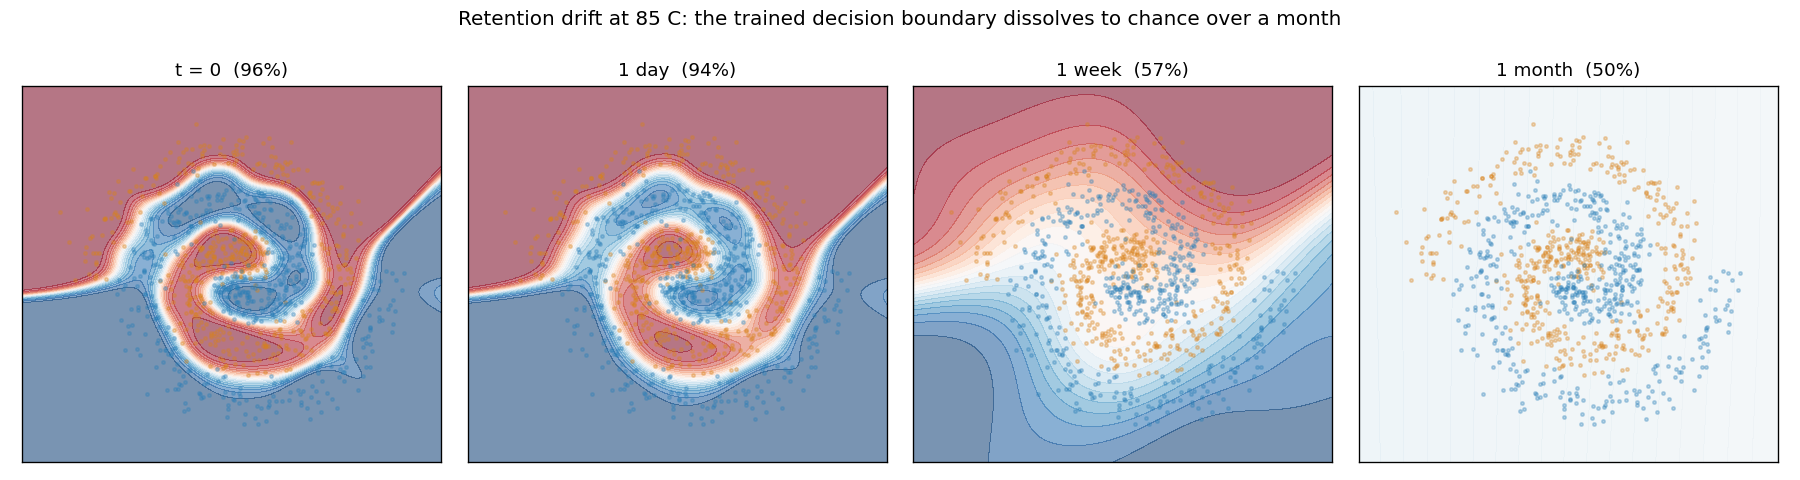
\includegraphics[width=0.98\textwidth]{figures/retention_boundary_strip.png}
\caption{The same trained network forgetting in time (frames left to right). As
the conductances relax at 85 degrees Celsius, the decision boundary is intact at
$t=0$ and after one day, washes out by one week (57 percent), and is gone by one
month (chance). No fixed set of weights can resist a time-varying decay.}
\label{fig:retstrip}
\end{figure*}

\section{Calibration, Operating Envelope, and Energy}
\label{sec:envelope}
The experiments so far use the generic device model. To ground the quantitative
conclusions in a real device and against an accepted baseline, we now calibrate
the model to a published cell, validate it, chart operating envelopes, and add an
energy model.

\textbf{Calibration to a published device.} We set the conductance window,
precision, rectification, and variability of the model to the measured Ag\textsubscript{2}O
self-rectifying 64x64 crossbar of Keshari et al. \cite{keshari2026}: a multilevel
window of 3.6 to 22.3 $\mu$S, more than four bits (16 levels), a rectification
ratio above $10^3$, and the negligible spatiotemporal variation they report. We
map a 784-128-10 MLP onto this device with differential pairs, 4-bit
quantization, and programming noise. Table \ref{tab:mnist} compares MNIST
accuracy: our calibrated simulator reaches $94.8 \pm 0.6$ percent, within about
one point of the measured 96.08 percent, and an established hardware-aware
inference toolkit (AIHWKit \cite{rasch2023}) on the same network gives
$95.4 \pm 0.2$ percent. The agreement validates the calibration and situates our
model among accepted tools.

\begin{table}[t]
\caption{MNIST (784-128-10 MLP) on the calibrated Ag\textsubscript{2}O device.}
\label{tab:mnist}
\centering
\begin{tabular}{lc}
\toprule
Method & Accuracy (\%) \\
\midrule
Software (float) & 95.70 \\
AIHWKit analog inference \cite{rasch2023} & $95.4 \pm 0.2$ \\
Our calibrated simulator (4-bit + variability) & $94.8 \pm 0.6$ \\
Keshari et al. 2026, measured \cite{keshari2026} & 96.08 \\
\bottomrule
\end{tabular}
\end{table}

\textbf{Operating envelopes.} Figure \ref{fig:envelope} charts, for the
calibrated device, where each remedy is needed. Panel (a) is the IR-drop envelope
over array size and wire resistance: below the 2 percent MVM-error contour naive
deployment suffices, between roughly 2 and 30 percent the loss is recoverable by
program-verify and in-situ training (Sections \ref{sec:res-inf},
\ref{sec:insitu}), and beyond it the array is IR-limited. Panel (b) is the
retention envelope over time and temperature, evaluated on the trained MLP: the
90 percent accuracy contour gives the rewrite cadence, which falls from years at
room temperature to days at 85 degrees. Together the two envelopes are a
predictive map: given a target accuracy, they bound the usable array size, wire
resistance, and rewrite interval.

One nuance worth stating: self-rectification, the headline feature of the
calibrated device, does \emph{not} reduce the read-time IR-drop error. In a fully
parallel single-ended MVM every cell is forward-biased, so the rectifying element
never engages; we verified that passive and self-rectifying cells give identical
MVM error (difference below 0.01 percent). Self-rectification suppresses
sneak-path and write-disturb currents and so enables denser passive arrays (the
benefit Keshari et al. emphasize), but the read-time IR drop is a wire-resistance
phenomenon it does not address. This separates two effects that are often
conflated.

\textbf{Energy.} Figure \ref{fig:energy} estimates compute efficiency. With the
calibrated conductances, a read pulse, and a per-column ADC, the array delivers
18 to 41 TOPS/W, rising with size as the ADC cost amortizes, against about 4
TOPS/W for a 0.5 pJ digital MAC. Energy therefore favors larger arrays, but the
IR-drop energy lost in the wires climbs from under 1 percent to 21 percent across
the same range, and IR drop also corrupts accuracy. The practical conclusion is
that the accuracy envelope of Fig. \ref{fig:envelope}(a), not energy, sets the
usable array size; within that envelope the calibrated device offers roughly five
to ten times the efficiency of the digital baseline.

\begin{figure*}[t]
\centering
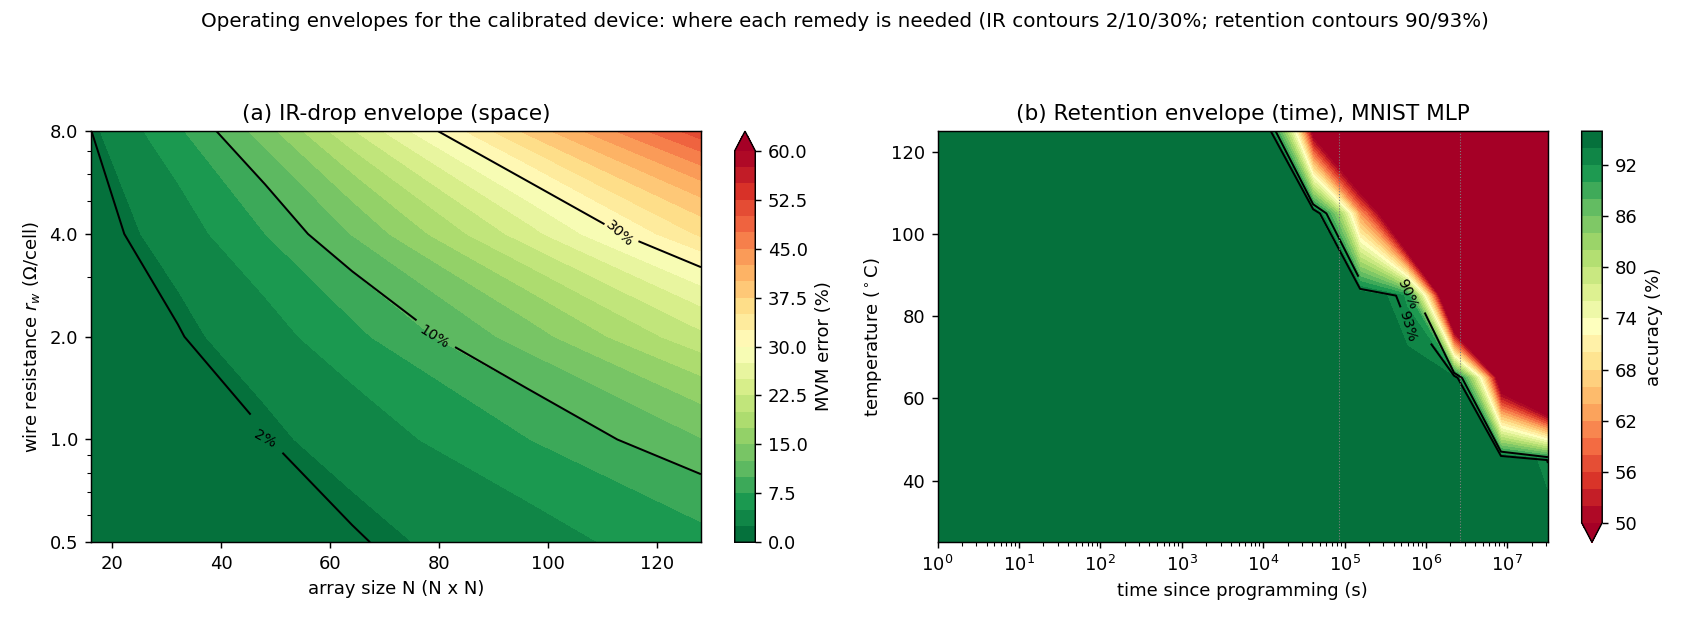
\includegraphics[width=0.98\textwidth]{figures/phase_diagram.png}
\caption{Operating envelopes for the calibrated Ag\textsubscript{2}O device.
(a) IR-drop envelope: mean MVM error over array size and wire resistance, with
2/10/30 percent contours marking the naive-OK, training-recoverable, and
IR-limited regions. (b) Retention envelope: accuracy of the trained MNIST MLP
over time and temperature, with 90/93 percent contours giving the rewrite cadence.}
\label{fig:envelope}
\end{figure*}

\begin{figure*}[t]
\centering
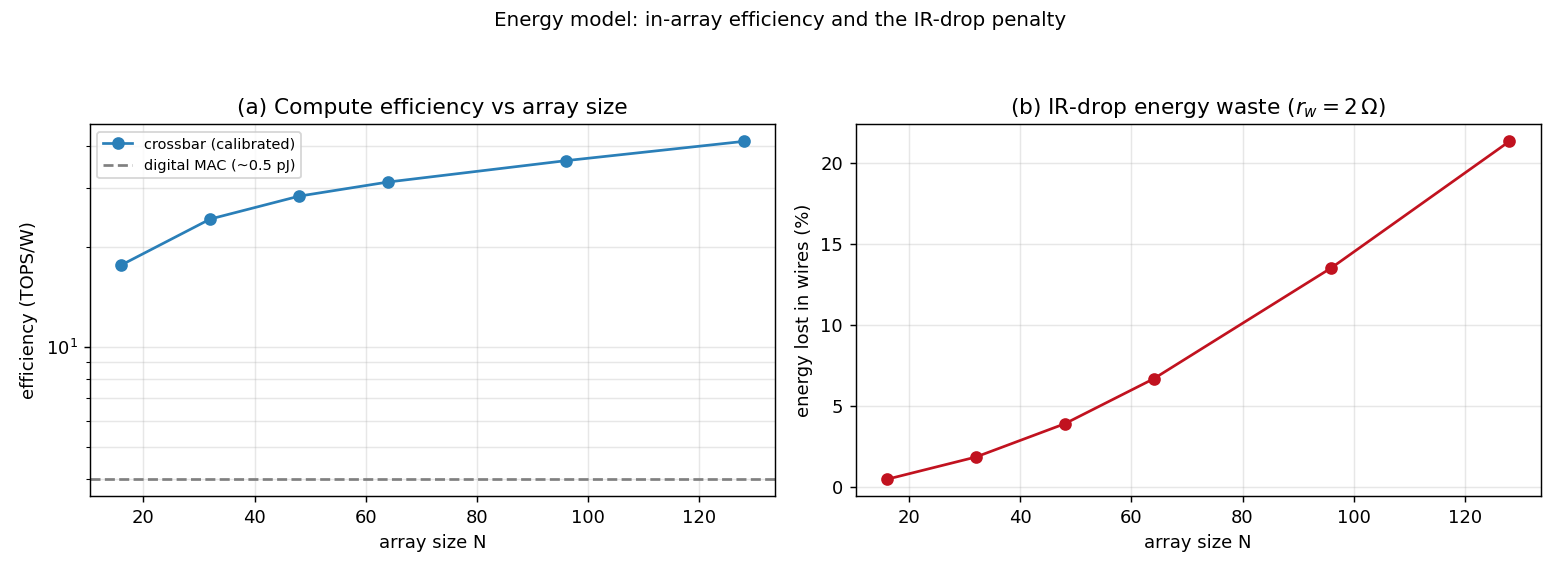
\includegraphics[width=0.92\textwidth]{figures/energy_model.png}
\caption{Energy model for the calibrated device. (a) Compute efficiency (TOPS/W)
versus array size, against a digital MAC reference. (b) Fraction of energy lost
in the wires to IR drop, which grows with array size.}
\label{fig:energy}
\end{figure*}

\section{Discussion: Separation by Remedy}
\label{sec:discussion}
Within this model and these tasks, the three non-idealities tend to separate by
the kind of remedy that helps, a separation made visible by holding the device
model fixed across all three:
\begin{itemize}
\item \textbf{Variability} behaves as a largely static, per-device offset, and is
\emph{correctable at write time} by closed-loop programming (program-verify
restores the classifier from $88.3$ to $96.5$ percent). This holds for the
programmable variation modeled here; stuck or non-responsive devices, read noise,
and limited verify budgets would leave a residual.
\item \textbf{IR drop} is a static, structured, input-dependent distortion of the
transfer function. It is not a write problem and program-verify does not fix it,
but it is largely \emph{absorbable by training} ($63.5$ to $92.4$ percent, versus
$69.3$ for output calibration alone), provided the array is not so resistive that
columns saturate. It still sets a practical ceiling on passive array size
(Table \ref{tab:irdrop}).
\item \textbf{Retention} is a time-varying decay, orthogonal to both: a fixed set
of trained weights cannot resist it, so it is \emph{deferred} by rewriting or
addressed by drift-aware mapping and recalibration, on a cadence set by the
activation energy and temperature.
\end{itemize}
The practical reading is that the three call for different mechanisms, and that
expecting one remedy to cover another (better programming to fix IR drop, or
one-time hardware-aware training to fix retention) is unlikely to work. We state
this as an observation under our model rather than a universal law.

\section{Limitations}
\label{sec:limitations}
This is a simulation study with a reduced model and several intentional
simplifications. The device model uses a single state variable and a simple
threshold rule; it captures hysteresis, multilevel states, frequency dependence,
and asymmetric updates, but not the full stochastic filament dynamics, read
disturb accumulation, or 1/f noise. The IR-drop study assumes a passive 1R array
and an all-LRS worst case for the scaling table; a 1T1R cell with an access
transistor would relax these numbers. Retention uses a single activation energy
and a relaxation toward the HRS; real distributions are broader. The in-situ
backward pass uses an ideal-weight surrogate gradient rather than a measured one;
the calibration baseline (Section \ref{sec:insitu}) shows the recovery is not a
trivial rescaling, but a measured or finite-difference gradient was not compared.
The tasks (digits, two spirals, circles) are small enough to fit a single tile;
we report a convolutional-layer fidelity rather than a full detector. We
calibrate to the \emph{reported} parameters of a published device (conductance
window, precision, rectification, variation) rather than fitting raw measured
I-V and retention curves, and the energy model is a first-order estimate (read
power plus a per-column ADC) without full peripheral, 1T1R, or interconnect
parasitics. None of the three underlying phenomena is itself novel; each is in
the literature of Section \ref{sec:relwork}. The contribution is the calibrated,
AIHWKit-baselined, seed-averaged study and the operating envelopes that make the
remedy boundaries quantitative. Remaining steps toward a top-venue result are
fitting the model to raw measured data, a full peripheral and 1T1R model with
silicon-grade energy, and larger networks.

\section{Conclusion}
Starting from one physically grounded oxide-memristor device equation, calibrated
to a published Ag\textsubscript{2}O cell, and scaling it without modification to a
64x64 array and a trained network, we gave a unified, seed-averaged account of
three crossbar non-idealities. Under this model they tend to separate by remedy:
variability is corrected at write time ($88.3$ to $96.5$ percent), IR drop is
absorbed by hardware-in-the-loop training ($63.5$ to $92.4$ percent, where output
calibration alone reaches only $69.3$), and retention is only deferrable. The
calibrated simulator reproduces the published 96.08 percent MNIST result to within
about a point and agrees with AIHWKit, and the resulting operating envelopes map
where each remedy is needed over array size, wire resistance, and temperature.
None of the underlying phenomena is individually new; the value is the calibrated,
baselined comparison and the predictive envelopes. Future work includes a 1T1R
access-device model, measured or finite-difference in-situ gradients, broader
retention-time distributions, fitting to raw measured device data, and larger
networks.

\section*{Acknowledgment}
This work, including both the simulation experiments and the writing of this
manuscript, was carried out with the assistance of Anthropic's Claude (Claude
Code). The author defined the research direction, made the key methodological
choices, and verified all results. A detailed provenance log distinguishing human
direction from AI-assisted execution is given in Appendix \ref{app:session}.

\begin{thebibliography}{00}
\bibitem{chua1971} L. O. Chua, ``Memristor: The missing circuit element,''
\textit{IEEE Trans. Circuit Theory}, vol. 18, no. 5, pp. 507--519, 1971.
\bibitem{strukov2008} D. B. Strukov, G. S. Snider, D. R. Stewart, and R. S.
Williams, ``The missing memristor found,'' \textit{Nature}, vol. 453, pp.
80--83, 2008.
\bibitem{ielmini2016} D. Ielmini, ``Resistive switching memories based on metal
oxides: mechanisms, reliability and scaling,'' \textit{Semicond. Sci. Technol.},
vol. 31, no. 6, p. 063002, 2016.
\bibitem{ielmini2018} D. Ielmini and H.-S. P. Wong, ``In-memory computing with
resistive switching devices,'' \textit{Nature Electronics}, vol. 1, pp.
333--343, 2018.
\bibitem{yu2018} S. Yu, ``Neuro-inspired computing with emerging nonvolatile
memories,'' \textit{Proc. IEEE}, vol. 106, no. 2, pp. 260--285, 2018.
\bibitem{yakopcic2011} C. Yakopcic, T. M. Taha, G. Subramanyam, R. E. Pino, and
S. Rogers, ``A memristor device model,'' \textit{IEEE Electron Device Lett.},
vol. 32, no. 10, pp. 1436--1438, 2011.
\bibitem{shafiee2016} A. Shafiee et al., ``ISAAC: A convolutional neural network
accelerator with in-situ analog arithmetic in crossbars,'' in \textit{Proc.
ISCA}, 2016, pp. 14--26.
\bibitem{chi2016} P. Chi et al., ``PRIME: A novel processing-in-memory
architecture for neural network computation in ReRAM-based main memory,'' in
\textit{Proc. ISCA}, 2016, pp. 27--39.
\bibitem{prezioso2015} M. Prezioso, F. Merrikh-Bayat, B. D. Hoskins, G. C.
Adam, K. K. Likharev, and D. B. Strukov, ``Training and operation of an
integrated neuromorphic network based on metal-oxide memristors,''
\textit{Nature}, vol. 521, pp. 61--64, 2015.
\bibitem{yao2020} P. Yao et al., ``Fully hardware-implemented memristor
convolutional neural network,'' \textit{Nature}, vol. 577, pp. 641--646, 2020.
\bibitem{li2018} C. Li et al., ``Analogue signal and image processing with large
memristor crossbars,'' \textit{Nature Electronics}, vol. 1, pp. 52--59, 2018.
\bibitem{liNComm2018} C. Li et al., ``Efficient and self-adaptive in-situ
learning in multilayer memristor neural networks,'' \textit{Nature
Communications}, vol. 9, 2385, 2018.
\bibitem{he2019} Z. He, J. Lin, R. Ewetz, J.-S. Yuan, and D. Fan, ``Noise
injection adaption: End-to-end ReRAM crossbar non-ideal effect adaption for
neural network mapping,'' in \textit{Proc. DAC}, 2019.
\bibitem{rasch2023} M. J. Rasch et al., ``Hardware-aware training for large-scale
and diverse deep learning inference workloads using in-memory computing-based
accelerators,'' \textit{Nature Communications}, vol. 14, 5282, 2023.
\bibitem{joshi2020} V. Joshi et al., ``Accurate deep neural network inference
using computational phase-change memory,'' \textit{Nature Communications}, vol.
11, 2473, 2020.
\bibitem{keshari2026} B. K. Keshari, C. K. R. Madadi, S. DebRoy, A. Salimath, V.
Mattela, and P. Sahatiya, ``Self-rectifying AgO-based synaptic crossbar array
for neuromorphic computing applications,'' \textit{Communications Materials},
2026, doi: 10.1038/s43246-026-01165-2.
\end{thebibliography}

\appendices
\section{Model Parameters and Implementation Notes}
\label{app:params}
Table \ref{tab:params} lists the default parameters used throughout. The array
draws $R_\mathrm{on}$ and $R_\mathrm{off}$ from log-normal distributions (so
resistances stay positive) and the thresholds from clipped Gaussians. The
small-signal read conductance at $V_\mathrm{read}$ is
$G_\mathrm{read}=I(V_\mathrm{read},w)/V_\mathrm{read}$, which is monotonic in $w$
and used for all weight reads.

\begin{table}[h]
\caption{Default device, array, and training parameters.}
\label{tab:params}
\centering
\small
\begin{tabular}{lll}
\toprule
Symbol & Meaning & Value \\
\midrule
$R_\mathrm{on}$ & LRS resistance (nominal) & $2\,\mathrm{k}\Omega$, $\sigma{=}15\%$ \\
$R_\mathrm{off}$ & HRS resistance (nominal) & $200\,\mathrm{k}\Omega$, $\sigma{=}30\%$ \\
$V_\mathrm{set}$ & SET threshold & $0.80$ V, $\sigma{=}0.08$ \\
$V_\mathrm{reset}$ & RESET threshold & $0.70$ V, $\sigma{=}0.08$ \\
$k_\mathrm{s},k_\mathrm{r}$ & switching rates & $80$ \\
$V_0$ & HRS nonlinearity scale & $0.45$ V \\
$p$ & window exponent & $4$ \\
$V_\mathrm{read}$ & read voltage & $0.2$ V \\
-- & cycle-to-cycle noise & $5\%$ \\
$[g_\mathrm{lo},g_\mathrm{hi}]$ & weight window & $[20,300]\,\mu$S \\
$E_a,\tau_0$ & retention (Arrhenius) & $1.0$ eV, $4.8{\times}10^{-9}$ s \\
$w_\mathrm{eq}$ & retention equilibrium & $0.02$ \\
$H$ & hidden units (spiral MLP) & $64$ \\
$w_\mathrm{max}$ & weight window (training) & $10$ \\
-- & batch size; float LR & $32$; $0.3$ \\
-- & pulse LR; max pulse width & $1.5{\times}10^{-3}$; $3{\times}10^{-3}$ \\
-- & IR-train epochs; LR decay & $350$; $0.992$ \\
$r_w$ & wire resistance (IR-train) & $1\,\Omega$/cell \\
\bottomrule
\end{tabular}
\end{table}

\textbf{IR-drop solver.} For an $N\times M$ array there are $2NM$ node voltages
(a row-wire and a column-wire node per cross-point). Assembly is fully
vectorized: device edges, row-wire edges, and column-wire edges are built as
index arrays, the diagonal is accumulated with \texttt{bincount}, and a single
sparse matrix is factored with \texttt{scipy.sparse.linalg.splu}. The same
factorization is reused for every input vector in a batch, which is what makes
hardware-in-the-loop training affordable.

\textbf{Differential decode.} With input voltages $V_\mathrm{in}=x\,V_\mathrm{read}$
and a differential pair encoding $W$, the recovered pre-activation is
$(I^{+}-I^{-})/(\text{decode scale}\cdot V_\mathrm{read})$, which equals $xW$ in
the ideal case; this identity was used to verify the inference pipeline (ideal
write reproduces the software accuracy in Table \ref{tab:inference}).

\section{Session Provenance Log}
\label{app:session}
Following the project's research protocol, we log what was human direction and
what was AI-assisted execution. The research was conducted as an interactive
session in which the human set the direction at each step and verified outcomes,
and the AI assistant (Claude Code) wrote and debugged the simulation code,
produced the figures, and drafted this manuscript. The work was not a
pre-registered plan; it grew turn by turn, which is why the appendix records the
actual order.

\subsection{Human Direction (verbatim prompts, in order)}
\begin{enumerate}
\item ``explain how neuromorphic memristor works''
\item ``lets say we're using AlOx -- i would like to visualize current-voltage
graph and see a simulation of a single device''
\item ``this is too much, i dont want animations, i want to scientifically
understand how the I-V hysteresis happens and how it helps to retain memory
state''
\item ``can you convert this to a script that simulates device level behaviour
and then create 64x64 crossbar array to see aggregate behaviour''
\item ``add wire-resistance IR-drop via a proper nodal solve (this is where 64x64
vs 128x128 starts to matter), model retention/drift as slow thermal relaxation of
w, run a small YOLO inference layer on the array to quantify accuracy loss from
variability''
\item ``if YOLO is too large, can you pick another demonstrable learning task
that can be shown to converge in this env itself, MNIST is too vanilla, also if
required increase the crossbar dims''
\item ``add retention drift between training and inference to see how fast a
trained network degrades, and train with IR-drop in the forward pass to see
whether the loop can learn around the wire resistance too''
\item ``can you somehow visualize the crossbar array and the weights encoded and
inference happening, like a test time inference''
\item ``run the same animation through the IR-drop forward, or animate the
retention drift''
\item ``generate another viz where the two tiles are receiving signals (how the
inputs are encoded to analog signals), and how the output is generated, visualize
the waveforms over time''
\item ``this viz isnt clear, can we make the efficiency takeaway much more
apparent and clear''
\item ``but i dont see the analog inputs coming into the crossbar array in
parallel''
\item ``treat this entire session as research, capture all the results and
generate a detailed paper, use IEEE format''
\end{enumerate}

\subsection{Mapping of Prompts to Outputs}
Table \ref{tab:provenance} maps each direction to the artifact the assistant
produced and the section of this paper that reports it.

\begin{table}[h]
\caption{Provenance: human direction to AI-produced artifact.}
\label{tab:provenance}
\centering
\small
\begin{tabular}{p{0.6cm}p{4.2cm}p{2.0cm}}
\toprule
Prompt & AI-produced artifact & Reported in \\
\midrule
1 & Conceptual explanation (no code) & -- \\
2 & Interactive device simulator (later set aside per prompt 3) & -- \\
3 & Written derivation of hysteresis and retention & Sec.~\ref{sec:device} \\
4 & \texttt{alox\_crossbar.py}: device model, 64x64 array & Fig.~\ref{fig:device}--\ref{fig:compute} \\
5 & \texttt{crossbar\_advanced.py}: MNA IR-drop, retention, conv + classifier & Fig.~\ref{fig:inference}--\ref{fig:retention}, Tab.~\ref{tab:irdrop} \\
6 & \texttt{crossbar\_learn.py}: in-situ two-spiral learning & Fig.~\ref{fig:insitu} \\
7 & Post-training drift; IR-drop in training loop & Fig.~\ref{fig:drift} \\
8--12 & Visualizations of encoding, MVM parallelism, signal flow & App.~\ref{app:extra} \\
13 & This manuscript & -- \\
\bottomrule
\end{tabular}
\end{table}

\subsection{Surprises and Debugging Insights}
Several non-obvious issues were found and fixed during execution; they are logged
here because they shaped the results.
\begin{itemize}
\item \textbf{Frequency collapse direction.} An early run showed the hysteresis
loop growing rather than shrinking with frequency, because the chosen rates let
the device fully switch at every tested frequency. Spacing the frequencies by
decades exposed the correct monotonic collapse (Fig.~\ref{fig:device}c).
\item \textbf{Inference decode bug.} The classifier first scored at chance
despite an ideal write; the cause was an input-voltage scale factor left out of
the differential decode while the bias was not scaled. Cosine similarity hid the
bug in the convolution check because it is scale invariant.
\item \textbf{Weight-range clipping.} In-situ learning stalled near 80 percent
until the conductance window was widened to encode weights up to about $\pm 8$;
the spiral network needs larger weights than a $\pm 3$ window allows.
\item \textbf{Noise as dither.} Noiseless identical devices stalled under
deterministic nonlinear updates, while cycle-to-cycle noise enabled convergence.
\item \textbf{Surrogate-gradient noise.} Hardware-in-the-loop IR-drop training
oscillated because the backward pass uses an ideal-weight surrogate; a pulse-size
decay schedule settled it (Fig.~\ref{fig:drift}c).
\end{itemize}

\subsection{Division of Labour}
Human contribution: the overall direction (start from device physics, scale to an
array, then add each non-ideality), the specific methodological asks (a proper
nodal solve, drift between training and inference, IR drop inside the training
loop, a non-trivial learning task), the decision to set aside an interactive
demo in favour of a reproducible script, and verification of each result. AI
contribution: implementation of the device and array models, the vectorized MNA
solver, the program-verify and in-situ training loops, all figures, the debugging
listed above, and the drafting of this paper. All numerical results were produced
by the released code and inspected by the human before inclusion.

\section{Additional Visualizations}
\label{app:extra}
Figure \ref{fig:compute} (referenced from Section \ref{sec:res-inf}) shows the
program-and-read of an image into the array and the analog MVM scatter.
Figures \ref{fig:parallel} and \ref{fig:circuit} are stills from animations built
to communicate the in-memory parallelism: the first contrasts the $N\times M$
sequential multiply-accumulate of a von Neumann engine with the single parallel
read of the crossbar; the second shows the analog inputs entering all wordlines
simultaneously and current summing down all bitlines at once.

\begin{figure}[t]
\centering
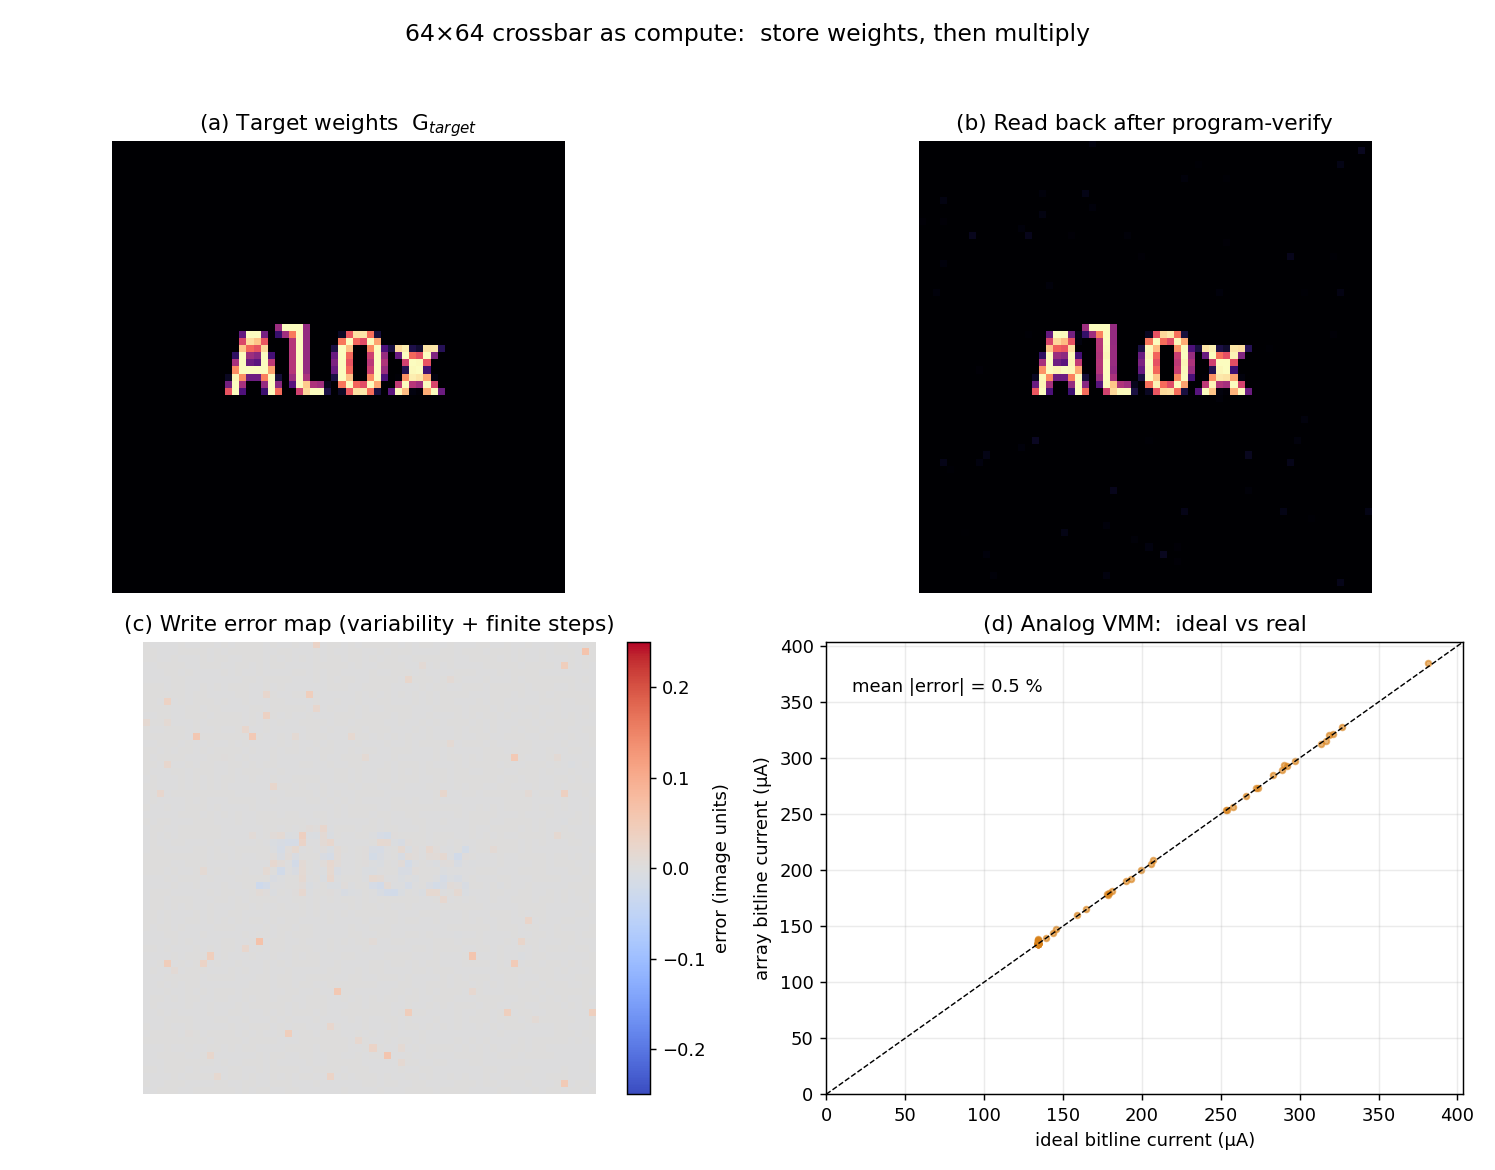
\includegraphics[width=\columnwidth]{figures/fig3_crossbar_compute.png}
\caption{Crossbar as compute. (a) Target weights (an image) and (b) the array
read-back after program-verify. (c) Write-error map. (d) Analog MVM versus ideal,
about 0.5 percent mean error.}
\label{fig:compute}
\end{figure}

\begin{figure*}[t]
\centering
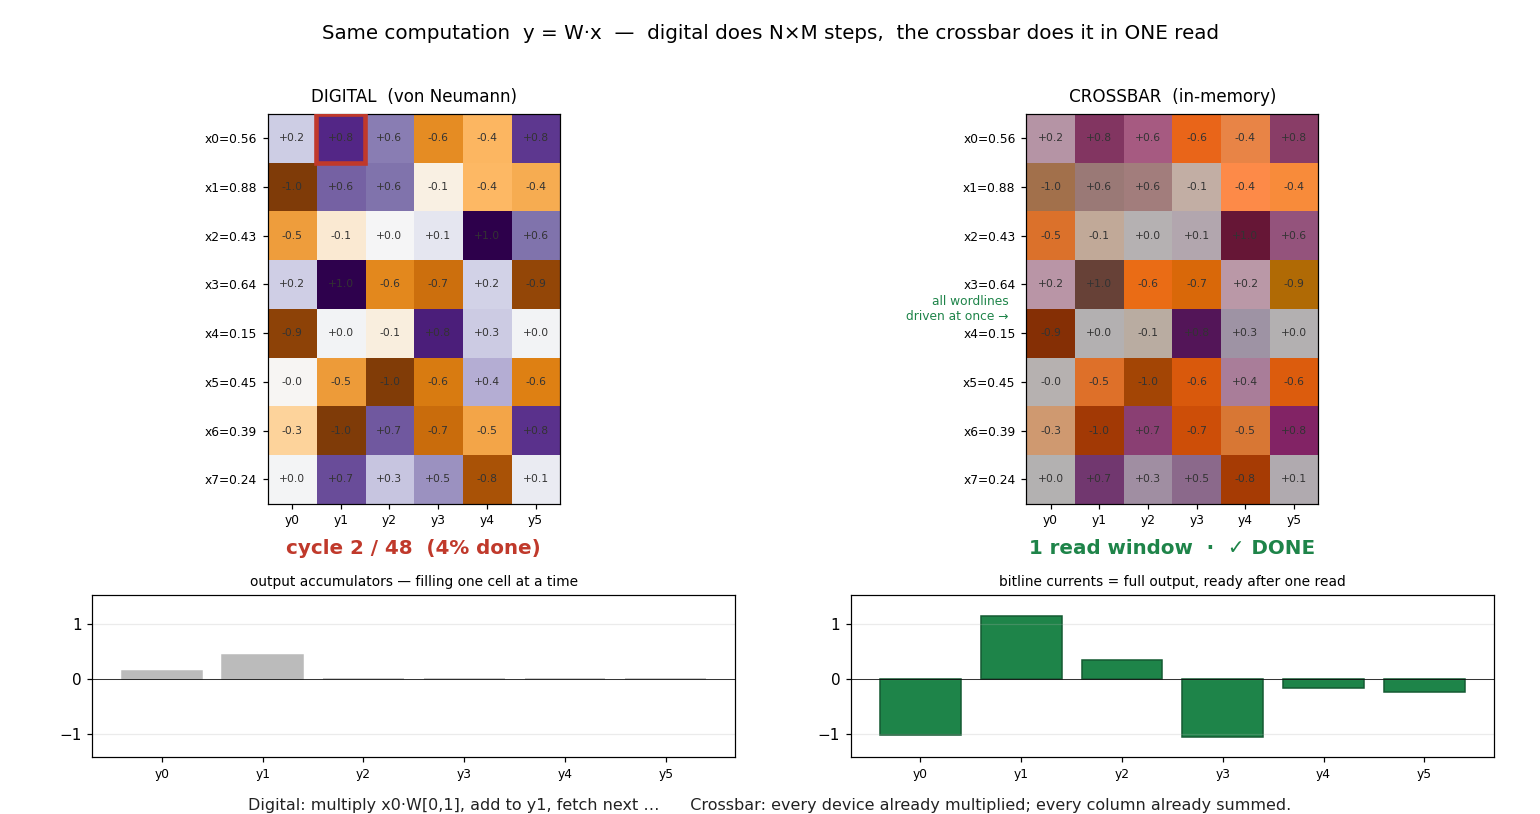
\includegraphics[width=0.32\textwidth]{figures/crossbar_parallel_f1.png}\hfill
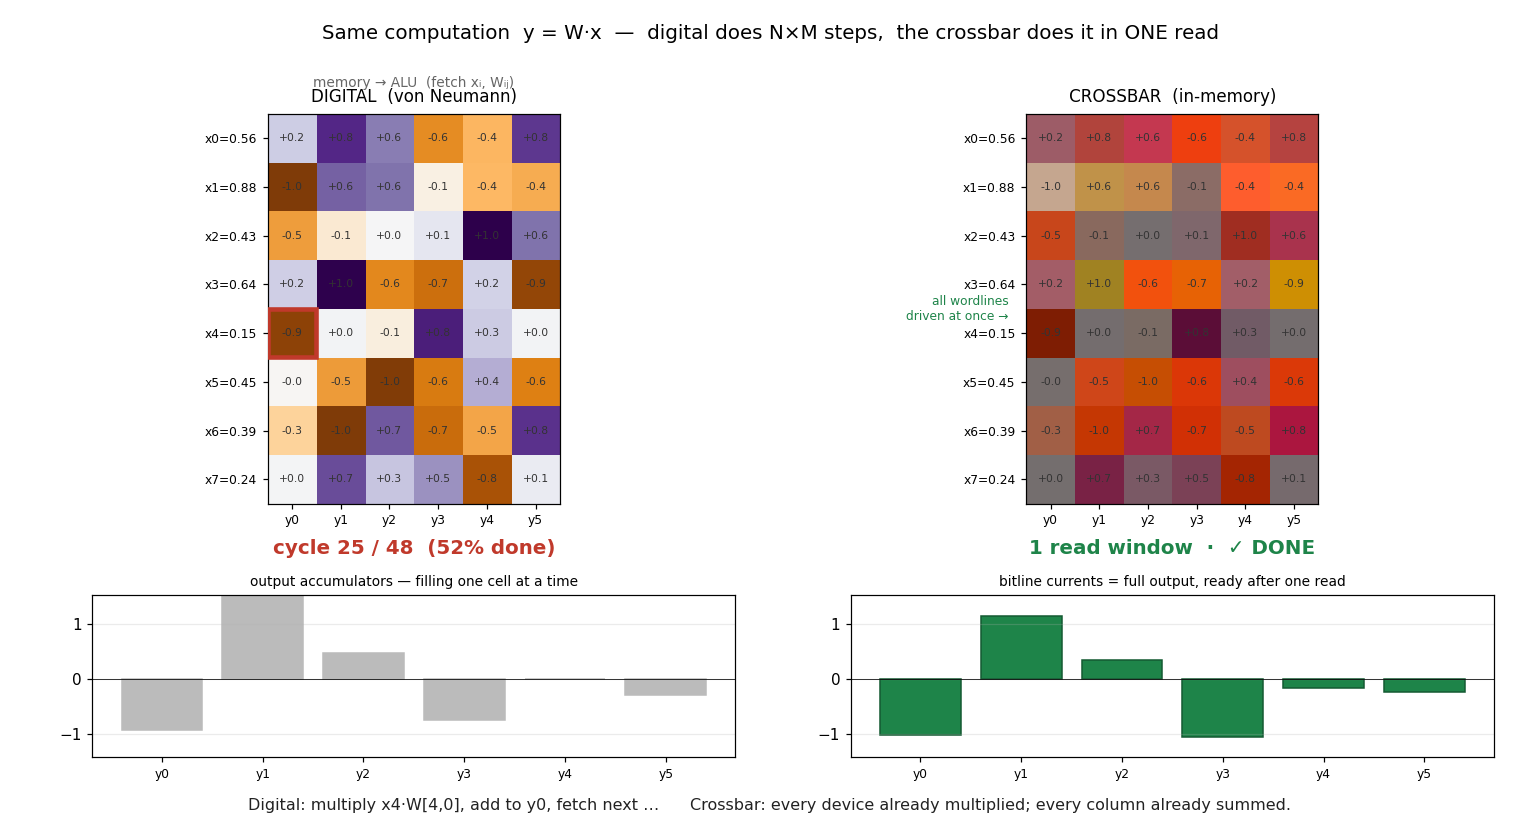
\includegraphics[width=0.32\textwidth]{figures/crossbar_parallel_f2.png}\hfill
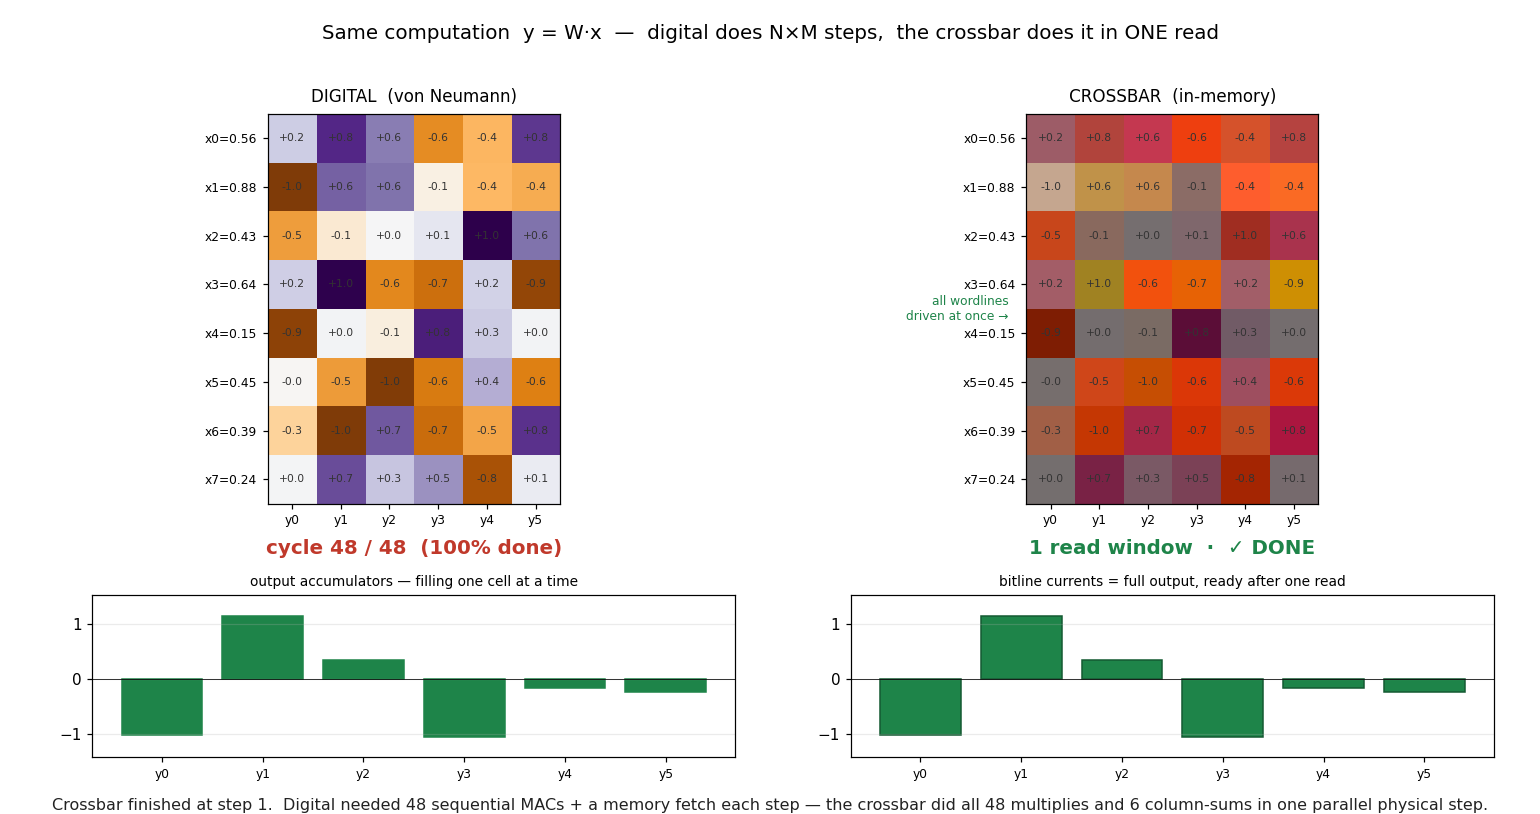
\includegraphics[width=0.32\textwidth]{figures/crossbar_parallel_f3.png}
\caption{The same MVM done two ways, shown at three times (left to right). The
digital engine steps through $N\times M$ multiply-accumulates with a memory fetch
each cycle (its counter climbs 1, mid, $N\times M$); the crossbar finishes the
whole product in one parallel read at step 1 and then holds the answer.}
\label{fig:parallel}
\end{figure*}

\begin{figure*}[t]
\centering
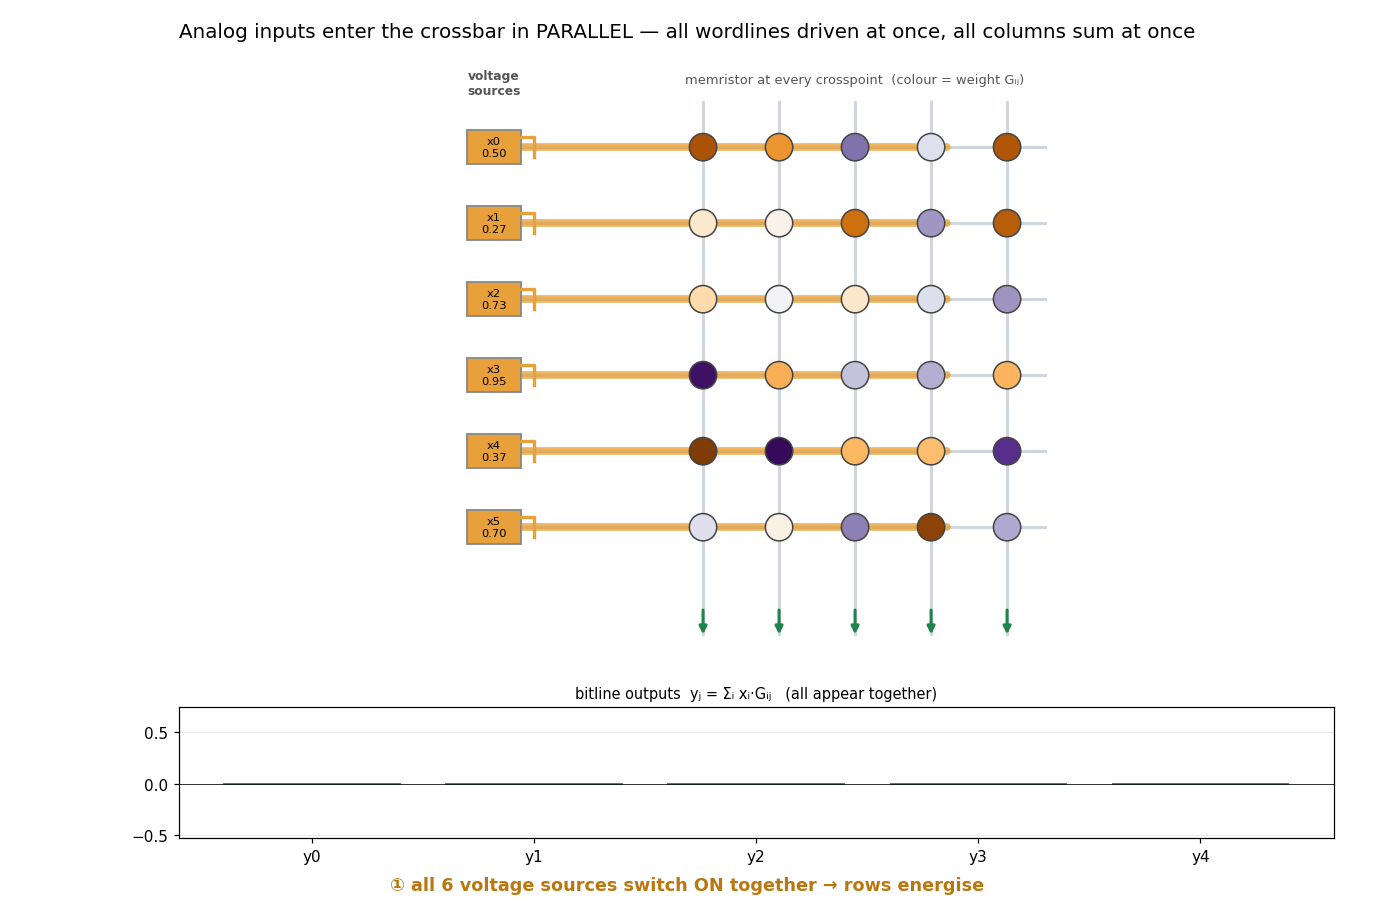
\includegraphics[width=0.32\textwidth]{figures/crossbar_circuit_f1.png}\hfill
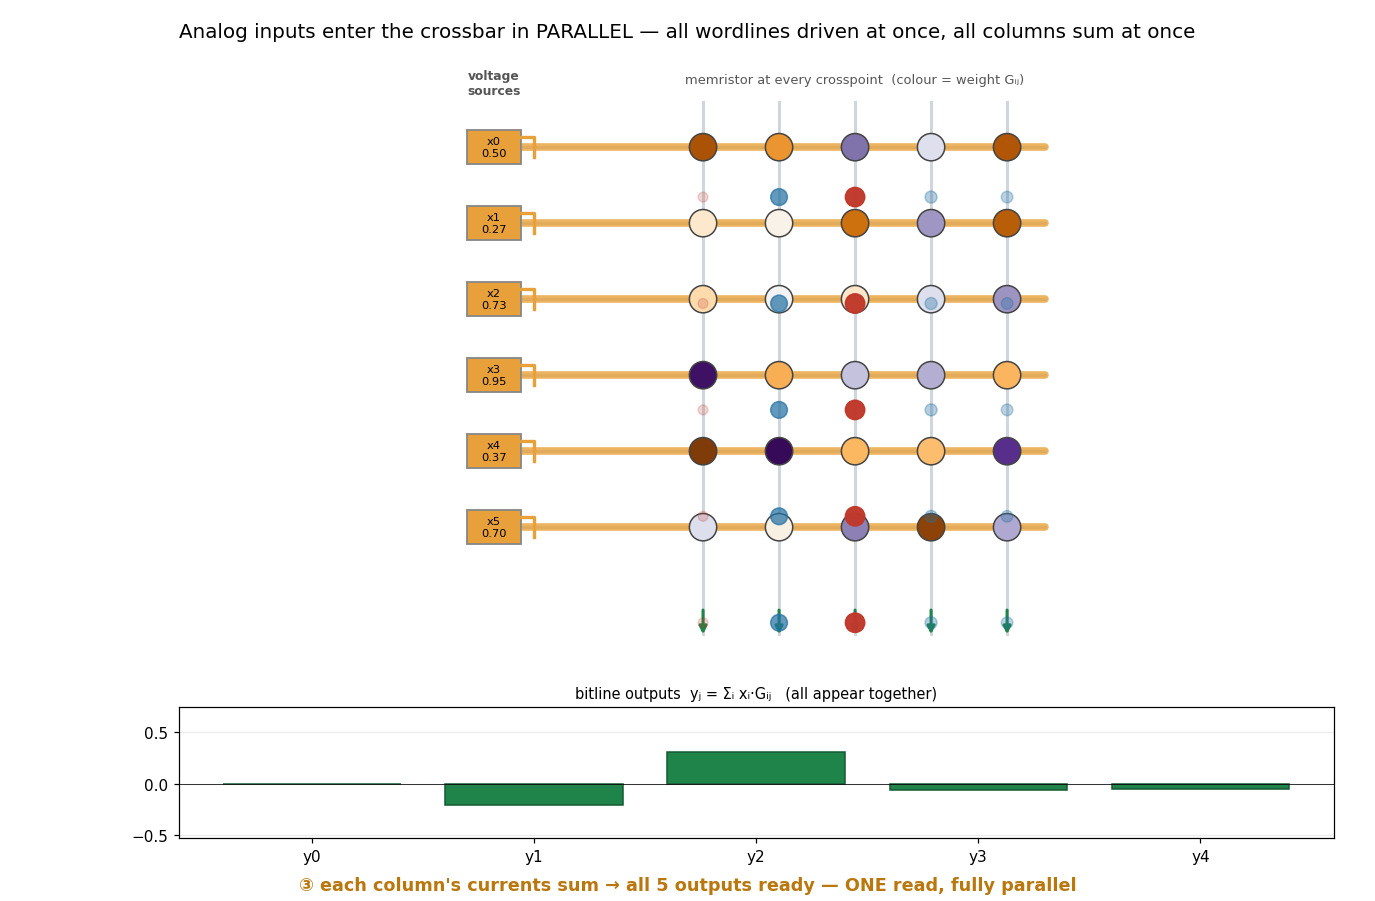
\includegraphics[width=0.32\textwidth]{figures/crossbar_circuit_f2.png}\hfill
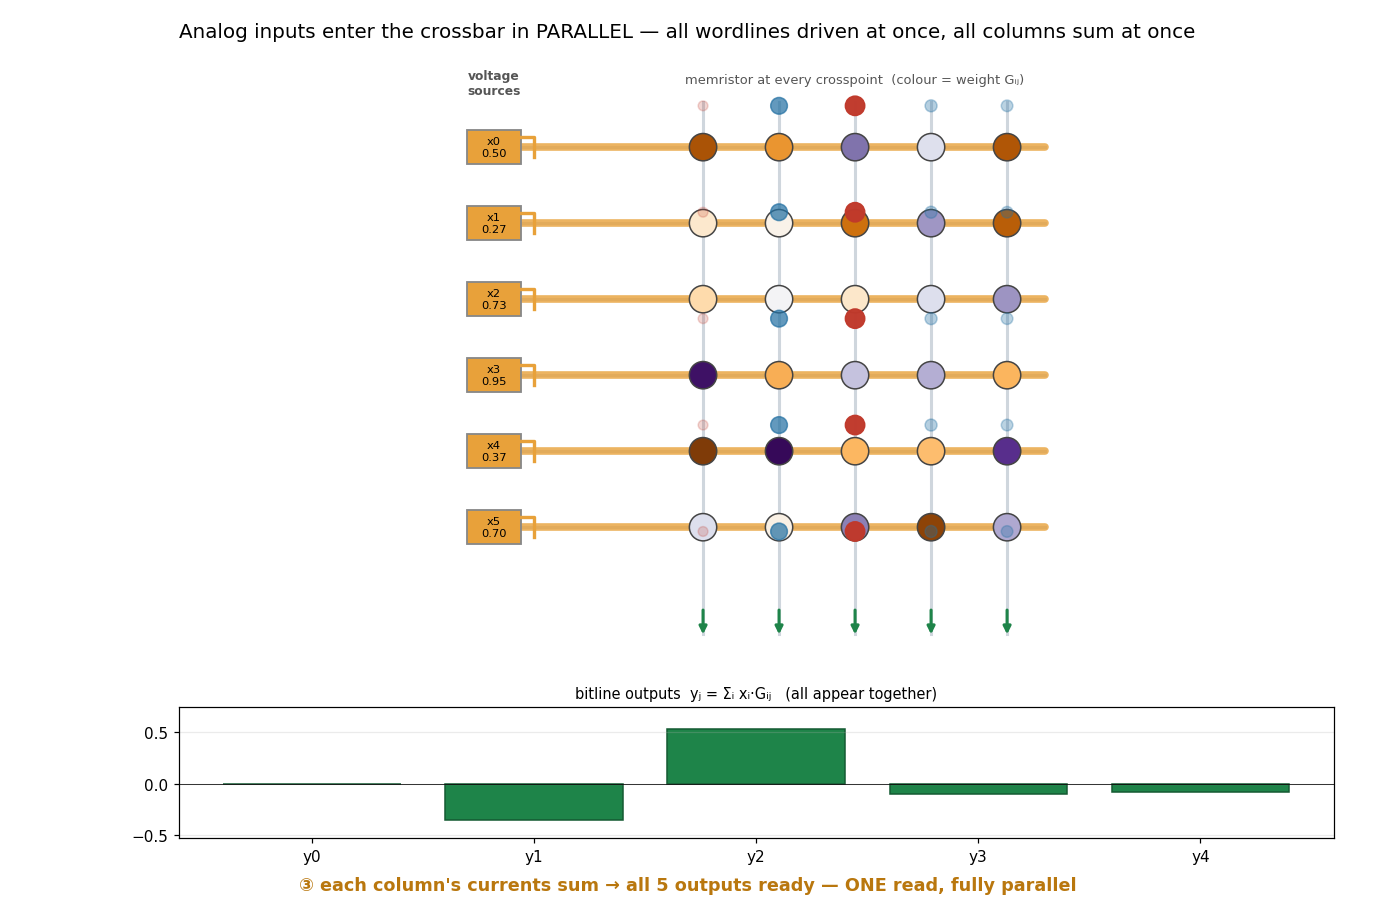
\includegraphics[width=0.32\textwidth]{figures/crossbar_circuit_f3.png}
\caption{Analog inputs entering the crossbar in parallel, shown at three times
(left to right): all wordlines are driven at once, every device passes $I=VG$,
and current then sums down every bitline simultaneously into the outputs.}
\label{fig:circuit}
\end{figure*}

\section{Reproducibility}
\label{app:repro}
All code accompanying this paper is in the public GitHub repository
\url{https://github.com/rayjyotir5/alox-crossbar-nonidealities} (Python 3.11;
NumPy, SciPy, scikit-learn, PyTorch, Matplotlib). It consists of three core
modules and several scripts:
\begin{itemize}
\item \texttt{alox\_crossbar.py}: device model, single-device sweep, 64x64 array
variability, image program/read, analog MVM (Fig.~\ref{fig:device}--\ref{fig:compute}).
\item \texttt{crossbar\_advanced.py}: vectorized MNA IR-drop solver, Arrhenius
retention, convolutional-layer fidelity, and the digit-classifier accuracy study
(Fig.~\ref{fig:inference}--\ref{fig:retention}, Tab.~\ref{tab:irdrop}).
\item \texttt{crossbar\_learn.py}: in-situ two-spiral training, hardware-in-the-loop
IR-drop training, and post-training retention (Fig.~\ref{fig:insitu}--\ref{fig:drift}).
\item \texttt{seeds\_experiments.py} and \texttt{harden2.py}: the multi-seed
study (classifier, in-situ on spirals and circles), the mixed-state IR-drop
table, the Arrhenius $E_a$ sensitivity, and the output-calibration baseline for
the IR-drop recovery. All headline numbers in the paper are produced here as
mean $\pm$ std over seeds.
\item Visualization scripts (\texttt{crossbar\_*\_viz.py}) produce the animations
whose stills appear in App.~\ref{app:extra}.
\end{itemize}
Each module is self-contained and writes its figures on execution; the full
pipeline runs in minutes on a single laptop CPU. Each headline result is reported
over multiple seeds (typically five for fast experiments, three for the slower
IR-aware training runs); the figures show a single representative seed while the
tables and text report the seed statistics.


\end{document}
